\documentclass[a4paper,12pt]{report}
%adaugat acum
\usepackage{fancyhdr}
\usepackage{lipsum}
%****%
\usepackage[romanian]{babel}
\usepackage{blindtext}
\usepackage{nameref}
\usepackage{hyperref}
\usepackage{amsmath}
\usepackage{tabu}
\usepackage{amssymb} 
\usepackage[utf8]{inputenc}
%\usepackage[left=3cm, top=2cm, right=2cm, bottom=2cm]{geometry}
\usepackage[left=2.5cm, top=2.5cm, right=2.5cm, bottom=2.5cm]{geometry}
\renewcommand{\baselinestretch}{1.5}
\usepackage{mathptmx}
\usepackage{titlesec}
\usepackage{esvect}
\usepackage{graphicx}
\usepackage{caption}
\usepackage[nottoc]{tocbibind}
\usepackage{amsmath,amssymb}
\DeclareMathOperator{\Exists}{\exists}
\DeclareMathOperator{\Forall}{\forall}
\newcommand\tab[1][1cm]{\hspace*{#1}}
\titleformat{\chapter}[display]
{\normalfont\large\bfseries\centering}{\chaptertitlename\ \thechapter}{0pt}{\Huge}
% this alters "before" spacing (the second length argument) to 0
\titlespacing*{\chapter}{0pt}{0pt}{20pt}

\fancypagestyle{plain}{%
  \renewcommand{\headrulewidth}{0pt}%
  \fancyhf{}%
}

\pagestyle{fancy}
\fancyfoot{}
\fancyhead[RO,LE]{\thepage}
\fancyhead[LO]{\leftmark}
\fancyhead[RE]{\rightmark}


\begin{document}

\begin{titlepage}
	\begin{center}
	\centering
	{\scshape\Large UNIVERSITATEA DIN BUCUREȘTI\\FACULTATEA DE MATEMATICĂ ȘI INFORMATICĂ\par}
	{\scshape\Large SPECIALIZAREA TEHNOLOGIA INFORMAȚIEI\par}
	\vspace{3cm}
	{\Huge\bfseries Lucrare de licență \par}
	\vspace{1cm}	
	{\Huge\bfseries CORECTAREA AUTOMATĂ A TESTELOR GRILĂ\par}
	\vspace{3.5cm}
	\end{center}
	{\large Coordonator stiințific: \\ Conf. univ. dr. Bogdan ALEXE\par}
	\vspace{1cm}
	{\large \tab \tab \tab \tab \tab  \tab \tab \tab \tab \tab  \tab \tab \tab \tab Absolvent: \\ \tab \tab  \tab  \tab   \tab  \tab    \tab \tab \tab \tab \hfill Ciprian-Mihai CEAUȘESCU}
	\vfill
	\centering
	% Bottom of the page
	{\large București, Iunie 2017}
\end{titlepage}


\chapter*{Abstract}
\vspace{2cm}
\tab În plină ascensiune tehnologică obiectivul urmărit de către cercetători este acela de a crea sisteme care să automatizeze procesele executate de către oameni. Domeniul \textit{inteligenței artificiale} își propune construirea de maşini inteligente care să modeleze sistemul de gândire și rațiune al individului. \textit{Vederea artificială}, subdomeniu al ramurii inteligenței artificiale, urmărește dezvoltarea de algoritmi capabili să reproducă funcționalitățile sistemului vizual uman. Lucrarea de față prezintă un proces automat de corectare a testelor grilă prin efectuarea unui set de operații asupra acestor teste în format digital. 
\\ \tab \\ \tab Un prim pas în realizarea acestui proces constă din extragerea grilelor existente în lucrare și detectarea pozițiilor pe care se găsesc răspunsurile alese de către elev sau student. Mașina de calcul trebuie să fie capabilă să parcurgă acest pas fără a întâmpina probleme.
\\ \tab \\ \tab În continuare, sistemul automat trece printr-o etapă de învățare supervizată. Tehnica utilizată este similară cu modalitatea abordată de către un profesor în școală care supervizează activitățile efectuate de către elevi. Astfel, se cunosc răspunsurile corecte pentru o anumită problemă, iar sistemul va face predicții asupra acestora, analizându-se totodată performanța obținută. Scopul acestei etape este acela de determinare automată a numărului grilei la care a răspuns elevul.
\\ \tab \\ \tab În final, rezultatele vor fi oferite către utilizatorul aplicației într-un format ușor de înțeles și analizat.

\chapter*{}

\chapter*{Abstract}
\vspace{2cm}
\tab Being a subject that is under constant development, scientists are looking to elaborate systems that can automate all the processes that were once executed by people. The \textit{artificial intelligence} field is set to build an intelligent machine that can understand how an individual thinks. \textit{Computer vision}, a subfield of artificial intelligence is developing some algorithms that will be able to simulate the functionalities of human visual system. This paper presents an automatic process of grading multiple choice tests by performing a set of operations on those tests on the computer. 
\\ \tab \\ \tab The first step is to take the grids from each paper and to detect the position of the answer that the student gave at the test. The computer must be able to perform this step without any errors.
\\ \tab \\ \tab The next step for the automated system is to go through supervised learning. The technique is similar to the way a teacher oversees the activities of his students. In this way, the system learns the right answers to a specific problem and will predict them. At the same time the results are analysed. This step should determin the number of the grid written on the test.
\\ \tab \\ \tab Lastly, the results will be returned to the user in a way that will be easily understood and analysed.

\chapter*{}

\tableofcontents{}

\chapter*{}

\listoffigures 
\tab \\
Figura 1.1 \hspace{2mm} Numărul de candidați în perioada 2012-2016\dotfill11\\
Figura 1.2 \hspace{2mm} Formatul lucrării de admitere\dotfill12\\
Figura 1.3 \hspace{2mm} Zona din lucrare unde se completează tipul grilei rezolvate\dotfill12\\
Figura 1.4 \hspace{2mm} Lucrare completată în sesiunea iulie 2016\dotfill13\\
Figura 1.5 \hspace{2mm} Schema procesului automat\dotfill14\\
Figura 2.1 \hspace{2mm} Filtru Gaussian de blurare de dimensiune $3\times3$\dotfill17\\
Figura 2.2 \hspace{2mm} Filtre convoluționale-derivatele parțiale în direcțiile x și y\dotfill18\\
Figura 2.3 \hspace{2mm} Rezultatele aplicării filtrelor convoluționale\dotfill18\\
Figura 2.4 \hspace{2mm} Calcularea magnitudinii gradientului\dotfill18\\
Figura 2.5 \hspace{2mm} Detectarea muchiilor\dotfill19\\
Figura 2.6 \hspace{2mm} Transformarea morfologică de închidere\dotfill20\\
Figura 2.7 \hspace{2mm} Transformarea morfologică de închidere\dotfill20\\
Figura 2.8 \hspace{2mm} Detecția contururilor\dotfill21\\
Figura 2.9 \hspace{2mm} Aplicarea algoritmului Ramer-Douglas-Peucker\dotfill21\\
Figura 2.10 \hspace{2mm} Calcularea HOG\dotfill23\\
Figura 2.11 \hspace{2mm} Calcularea descriptorului HOG\dotfill24\\
Figura 2.12 \hspace{2mm} Rezultatul calculării descriptorului HOG\dotfill24\\
Figura 2.13 \hspace{2mm} Separarea claselor de obiecte\dotfill25\\
Figura 2.14 \hspace{2mm} Determinarea hiperplanurilor\dotfill26\\
Figura 2.15 \hspace{2mm} Imagini din setul MNIST\dotfill26\\
Figura 2.16 \hspace{2mm} Matricea unei cifre din setul MNIST\dotfill26\\
Figura 2.17 \hspace{2mm} Tehnica învățării supervizate\dotfill27\\
Figura 3.1 \hspace{2mm} Tipuri de zgomot\dotfill29\\
Figura 3.2 \hspace{2mm} Eliminarea zgomotului cu o valoare de prag de 180\dotfill30\\
Figura 3.3 \hspace{2mm} Răspunsul filtrului Gaussian de dimensiune 5, respectiv 15\dotfill31\\
Figura 3.4 \hspace{2mm} Detecția muchiilor folosind Canny (imagine cu filtrul Gaussian)\dotfill31\\
Figura 3.5 \hspace{2mm} Detecția muchiilor folosind Canny (imagine fără filtrul Gaussian)\dotfill32\\
Figura 3.6 \hspace{2mm} Închiderea și evidențierea muchiilor folosind operația morfologică de închidere\dotfill32\\
Figura 3.7 \hspace{2mm} Reprezentarea contururilor detectate\dotfill33\\
Figura 3.8 \hspace{2mm} Coordonatele obținute în urma detecției colțurilor grilelor\dotfill34\\
Figura 3.9 \hspace{2mm} Grilele care au fost decupate din lucrare\dotfill35\\
Figura 3.10 \hspace{2mm} Zonele cu răspunsuri din grilele extrase\dotfill35\\
Figura 3.11 \hspace{2mm} Accentuarea detaliilor zonelor cu răspunsuri\dotfill36\\
Figura 3.12 \hspace{2mm} Matricea de răspunsuri rezultată\dotfill37\\
Figura 3.13 \hspace{2mm} Zona aferentă tipului grilei și a numărului variantei\dotfill37\\
Figura 3.14 \hspace{2mm} Zona accentuată a tipului grilei\dotfill38\\
Figura 3.15 \hspace{2mm} Rezultatul calculării HOG asupra imaginilor cu cifre\dotfill38\\
Figura 3.16 \hspace{2mm} Graficele HOG-urilor aferente imaginilor din figura 3.15\dotfill39\\
Figura 3.17 \hspace{2mm} Contururile detectate în zona numărului variantei\dotfill40\\
Figura 3.18 \hspace{2mm} Cifre extrase din lucrări ale setului de test\dotfill40\\
Figura 3.19 \hspace{2mm} Compararea răspunsurilor bifate cu cele corecte\dotfill41\\
Figura 4.1 \hspace{2mm} Imagini cu cifre din setul MNIST\dotfill47\\
Figura 4.2 \hspace{2mm} Imagini cu cifre din lucrări completate la examenul de admitere din iulie 2016\dotfill47\\
Figura 4.3 \hspace{2mm} Diferența dintre HOG 4 celule și 16 celule\dotfill51\\
\listoftables
\tab \\
Tabelul 4.1 \hspace{2mm} Verificarea valorilor pragului de eliminare al zgomotului\dotfill45\\
Tabelul 4.2 \hspace{2mm} Timpul mediu de execuție al corectării\dotfill46\\ 
Tabelul 4.3 \hspace{2mm} Timpul mediu de execuție al întregului proces pentru o lucrare\dotfill46\\  
Tabelul 4.4 \hspace{2mm} Timpul mediu de execuție al testelor\dotfill47\\  
Tabelul 4.5 \hspace{2mm} Acuratețe SVM folosind HOG 4 celule - teste MNIST\dotfill47\\  
Tabelul 4.6 \hspace{2mm} Acuratețe SVM folosind HOG 4 celule - teste lucrări 2016\dotfill48\\  
Tabelul 4.7 \hspace{2mm} Timpi de execuție antrenare MNIST și testare MNIST\dotfill48\\  
Tabelul 4.8 \hspace{2mm} Timpi de execuție antrenare MNIST și testare lucrări 2016\dotfill49\\  
Tabelul 4.9 \hspace{2mm} Acuratețe SVM folosind HOG 16 celule - teste MNIST\dotfill49\\  
Tabelul 4.10 \hspace{2mm} Acuratețe SVM folosind HOG 16 celule - teste lucrări 2016\dotfill50\\  
Tabelul 4.11 \hspace{2mm} Timpi de execuție antrenare MNIST și testare MNIST\dotfill50\\  
Tabelul 4.12 \hspace{2mm} Timpi de execuție antrenare MNIST și testare lucrări 2016\dotfill51\\  

\chapter*{}

\chapter{Introducere}
\tab În ultima vreme se observă faptul că tendințele din lumea tehnologiei sunt într-o continuă schimbare. Aceste schimbări vor influența modul în care 
noi, oamenii, vom folosi tehnologia. Accentul cade în special pe: cloud computing, mobilitate, social business, dar și pe conceptul foarte
important de big data. Susținerea acestor piloni este realizată de realitatea virtuală și augumentată, robotică, sisteme cognitive, dar și Internet of Things,
tehnologii importante care au ca nucleu de interes \textit{inteligența artificială}.  
\\ \tab În această lume a dezvoltării tehnologice, principalul obiectiv urmărit este acela de automatizare a proceselor realizate de către oameni.
Lucrarea de față propune un algoritm de corectare a testelor grilă, folosind o interfață grafică prietenoasă. Formatul acestor teste grilă este folosit
 la concursul de admitere la domeniul de studiu Calculatoare și Tehnologia Informației, specializarea Tehnologia Informației, din cadrul Facultății de Matematică și
Informatică, Universitatea din București. Pe piața industriei software există aplicații similare\cite{articol1, articol2}, dar care nu se pretează formatului lucrărilor utilizat la Facultatea de Matematică și Informatică.
\\ \tab De-a lungul timpului s-a observat o creștere considerabilă a numărului de elevi care optează pentru admiterea la domeniul de studiu Calculatoare și Tehnologia Informației, astfel
încât un proces automatizat pentru corectarea lucrărilor diminuează mult efortul comisiei de admitere. În figura 1.1 se prezintă un grafic corespunzător numărului de elevi care au candidat la concursul
de admitere în perioada 2012-2016:
\begin {center} 
	\begin {footnotesize} 
		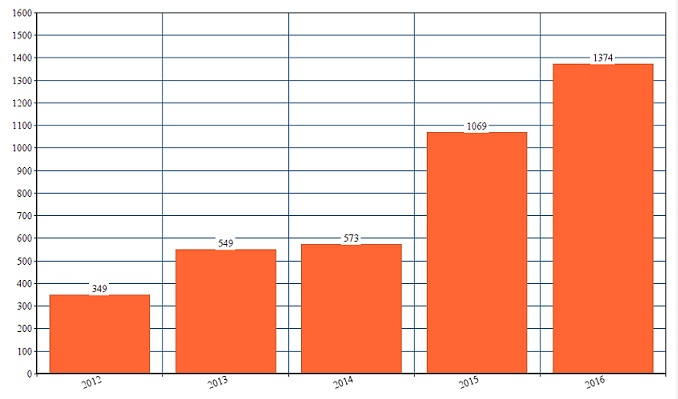
\includegraphics[width =104mm]{fig1_1}  \\
		\textbf  {Figura 1.1} Numărul de candidați în perioada 2012-2016
	\end {footnotesize} 
\end {center}
\tab Formatul lucrărilor de admitere care se folosesc în momentul de față la examen este prezentat în figura 1.2. Acesta are câteva zone importante, printre care colțul din dreapta sus în care se 
completează datele personale ale elevului și se sigilează, câmpurile din stânga unde se trece nota obținută la examen, respectiv partea de jos corespunzătoare zonelor în care se bifează răspunsurile elevului.
\begin {center} 
	\begin {footnotesize} 
		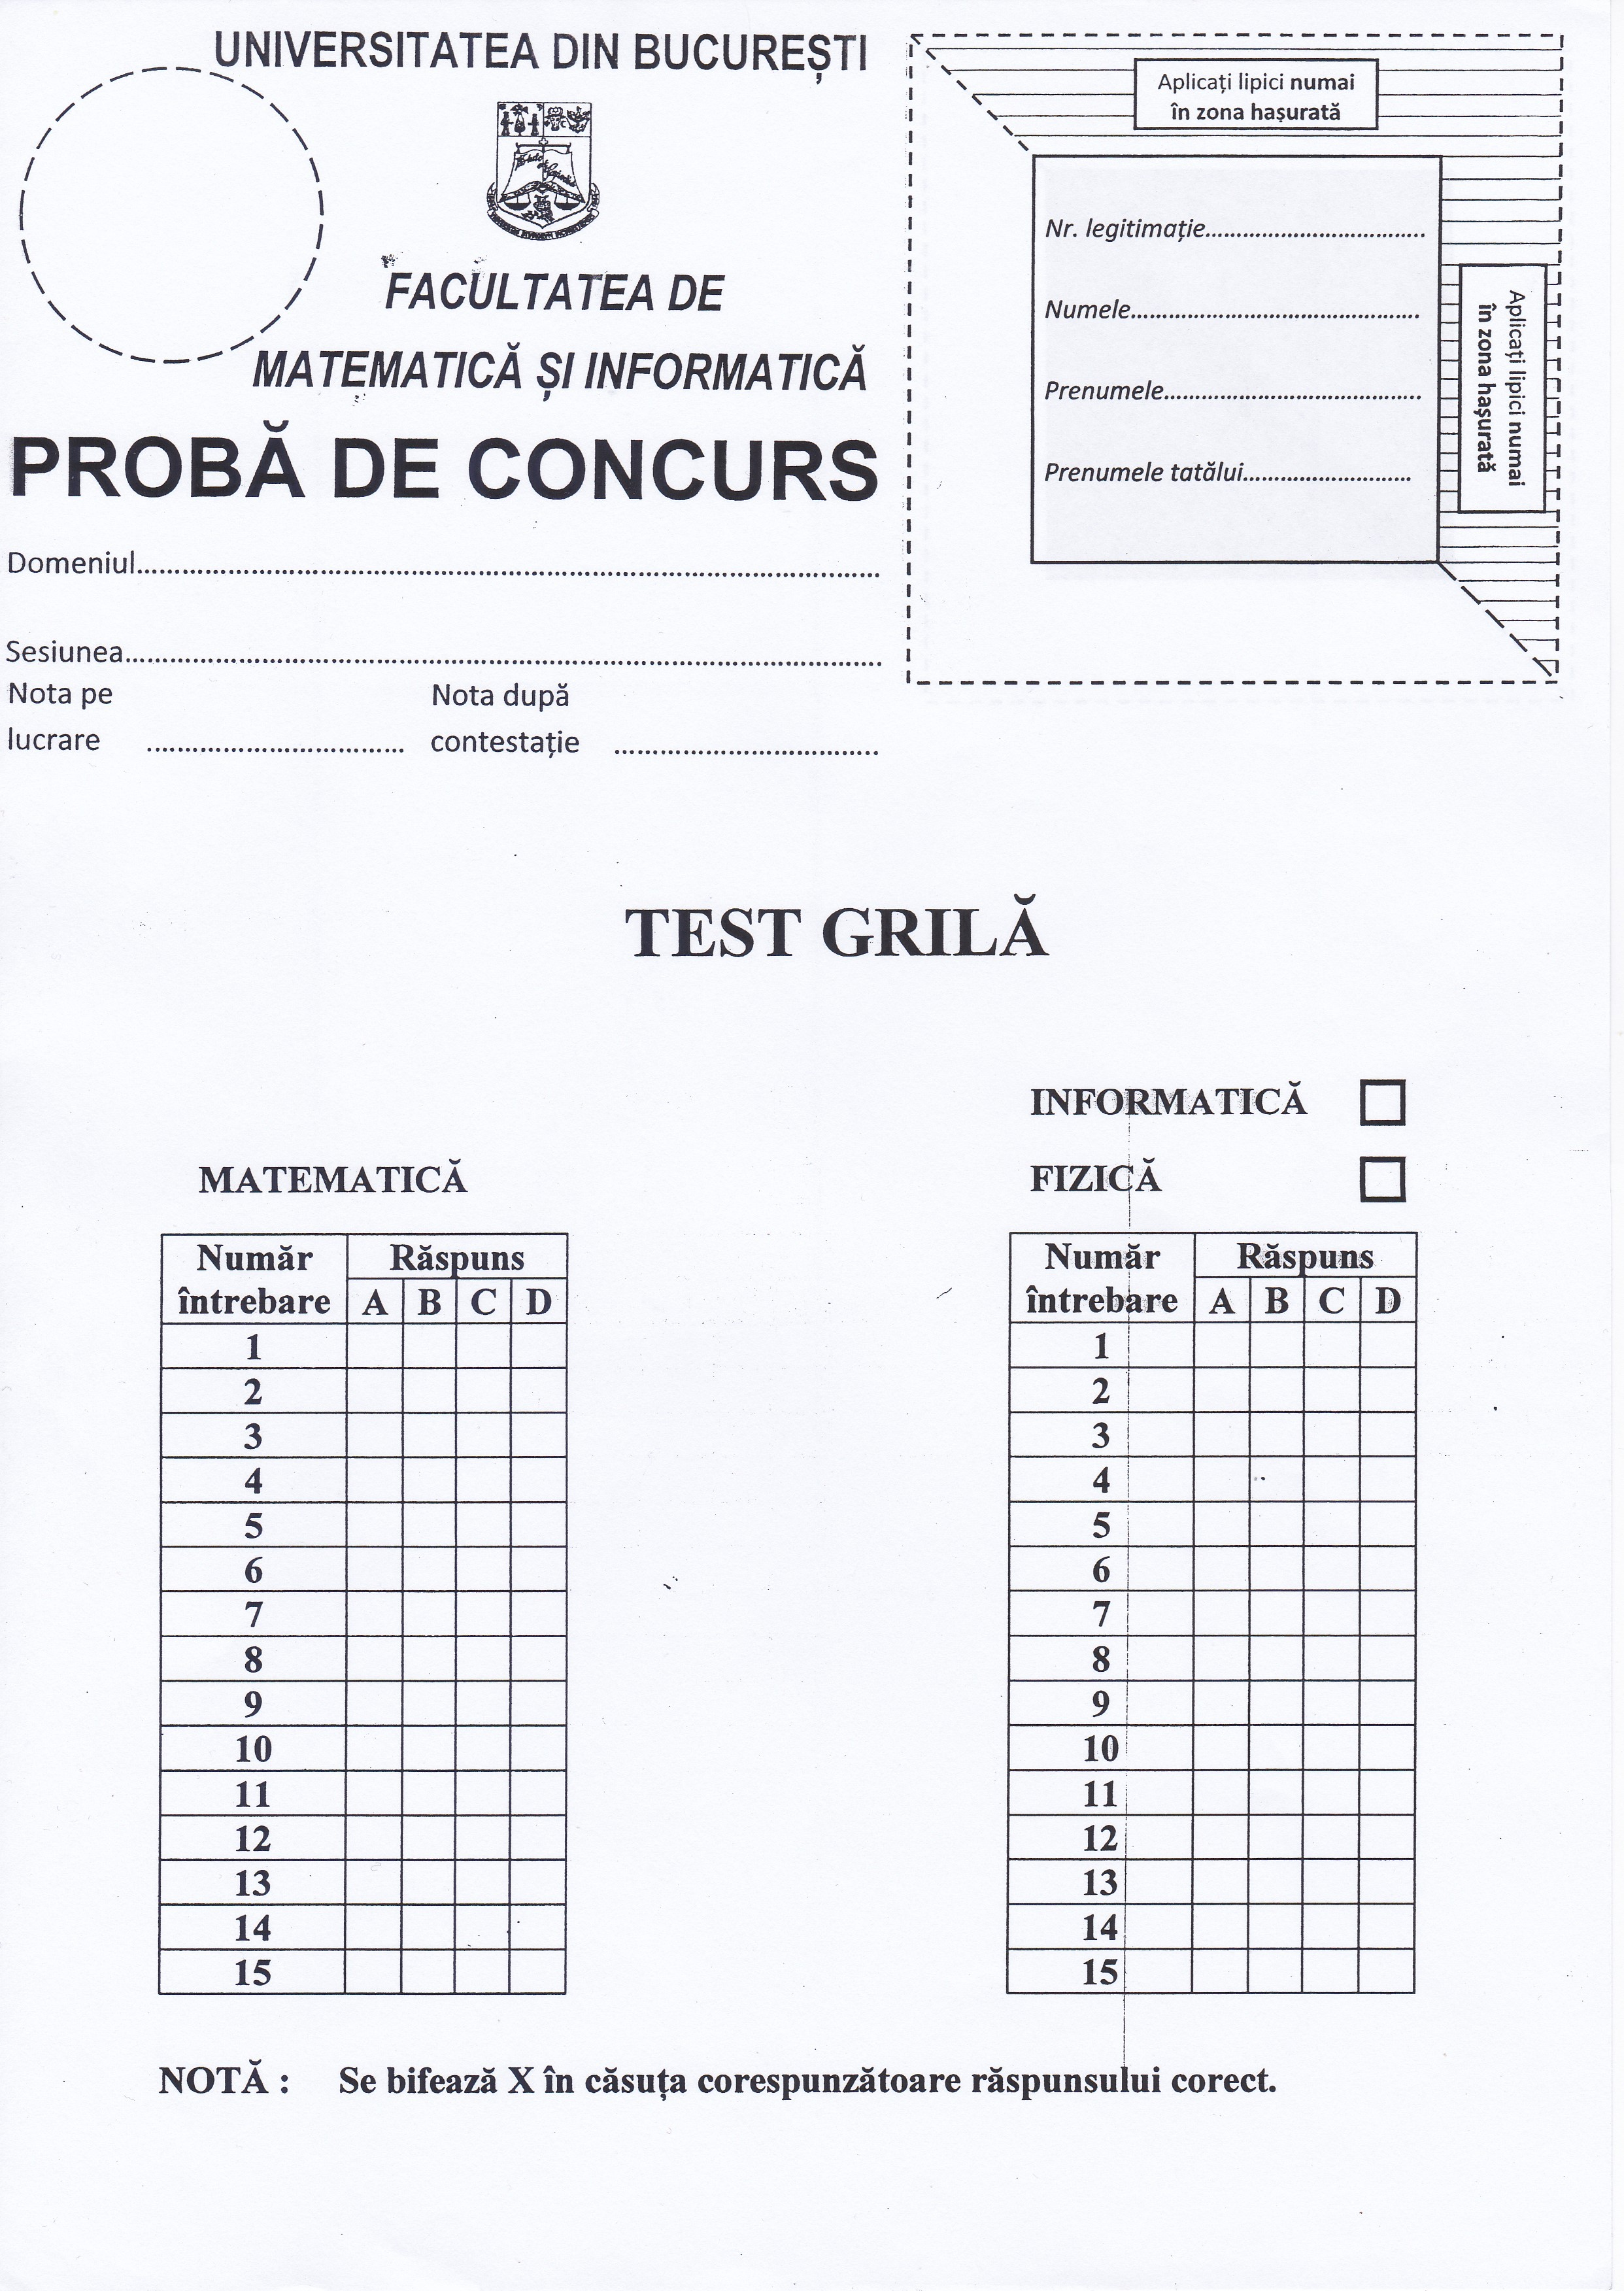
\includegraphics[width =67mm]{fig1_2}  \\
		\textbf  {Figura 1.2} Formatul lucrării de admitere
	\end {footnotesize} 
\end {center}
\tab În vederea elaborării subiectelor pentru examenul de admitere de la domeniul de studiu Calculatoare și Tehnologia Informației sunt realizate 4 tipuri de variante, numerotate de la 1 la 4. Fiecare variantă este formată din 3 subiecte, și anume, matematică,
informatică și fizică, dintre care elevul trebuie să rezolve obligatoriu grila de matematică și la alegere, grila de informatică sau fizică. În funcție de numărul subiectului pe care îl primește, dar și de opțiunea pe care o face, 
elevul completează în căsuța corespunzătoare alegerii sale, numărul variantei la care răspunde. De exemplu, dacă elevul primește varianta numărul 2 de subiect și optează pentru a rezolva grila de fizică, acesta completează în zona dedicată variantei de subiect, 
numărul corespunzător, conform figurii 1.3.
\begin {center} 
	\begin {footnotesize} 
		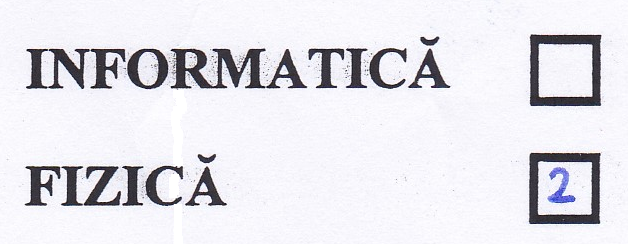
\includegraphics[width =55mm]{fig1_3} \\
		\textbf  {Figura 1.3} Zona din lucrare unde se completează tipul grilei rezolvate
	\end {footnotesize} 
\end {center}
\tab Lucrarea de examen pe care o primește elevul se completează de către acesta cu datele personale și se secretizează. De asemenea, se completează informații cu privire la domeniul pentru care a aplicat elevul, alături de
sesiunea în care a avut loc examinarea. Numărul variantei primite și tipul de grilă aleasă se trec în locul destinat acestor informații. Răspunsurile la întrebări se bifează pe foaia de concurs, în zona corespunzătoare, printr-un X, iar orice alt însemn pe foaia
de examinare duce la respingerea lucrării de către comisia de admitere. Un exemplu de lucrare completată în mod corespunzător este prezentat în figura 1.4.
\begin {center} 
	\begin {footnotesize} 
		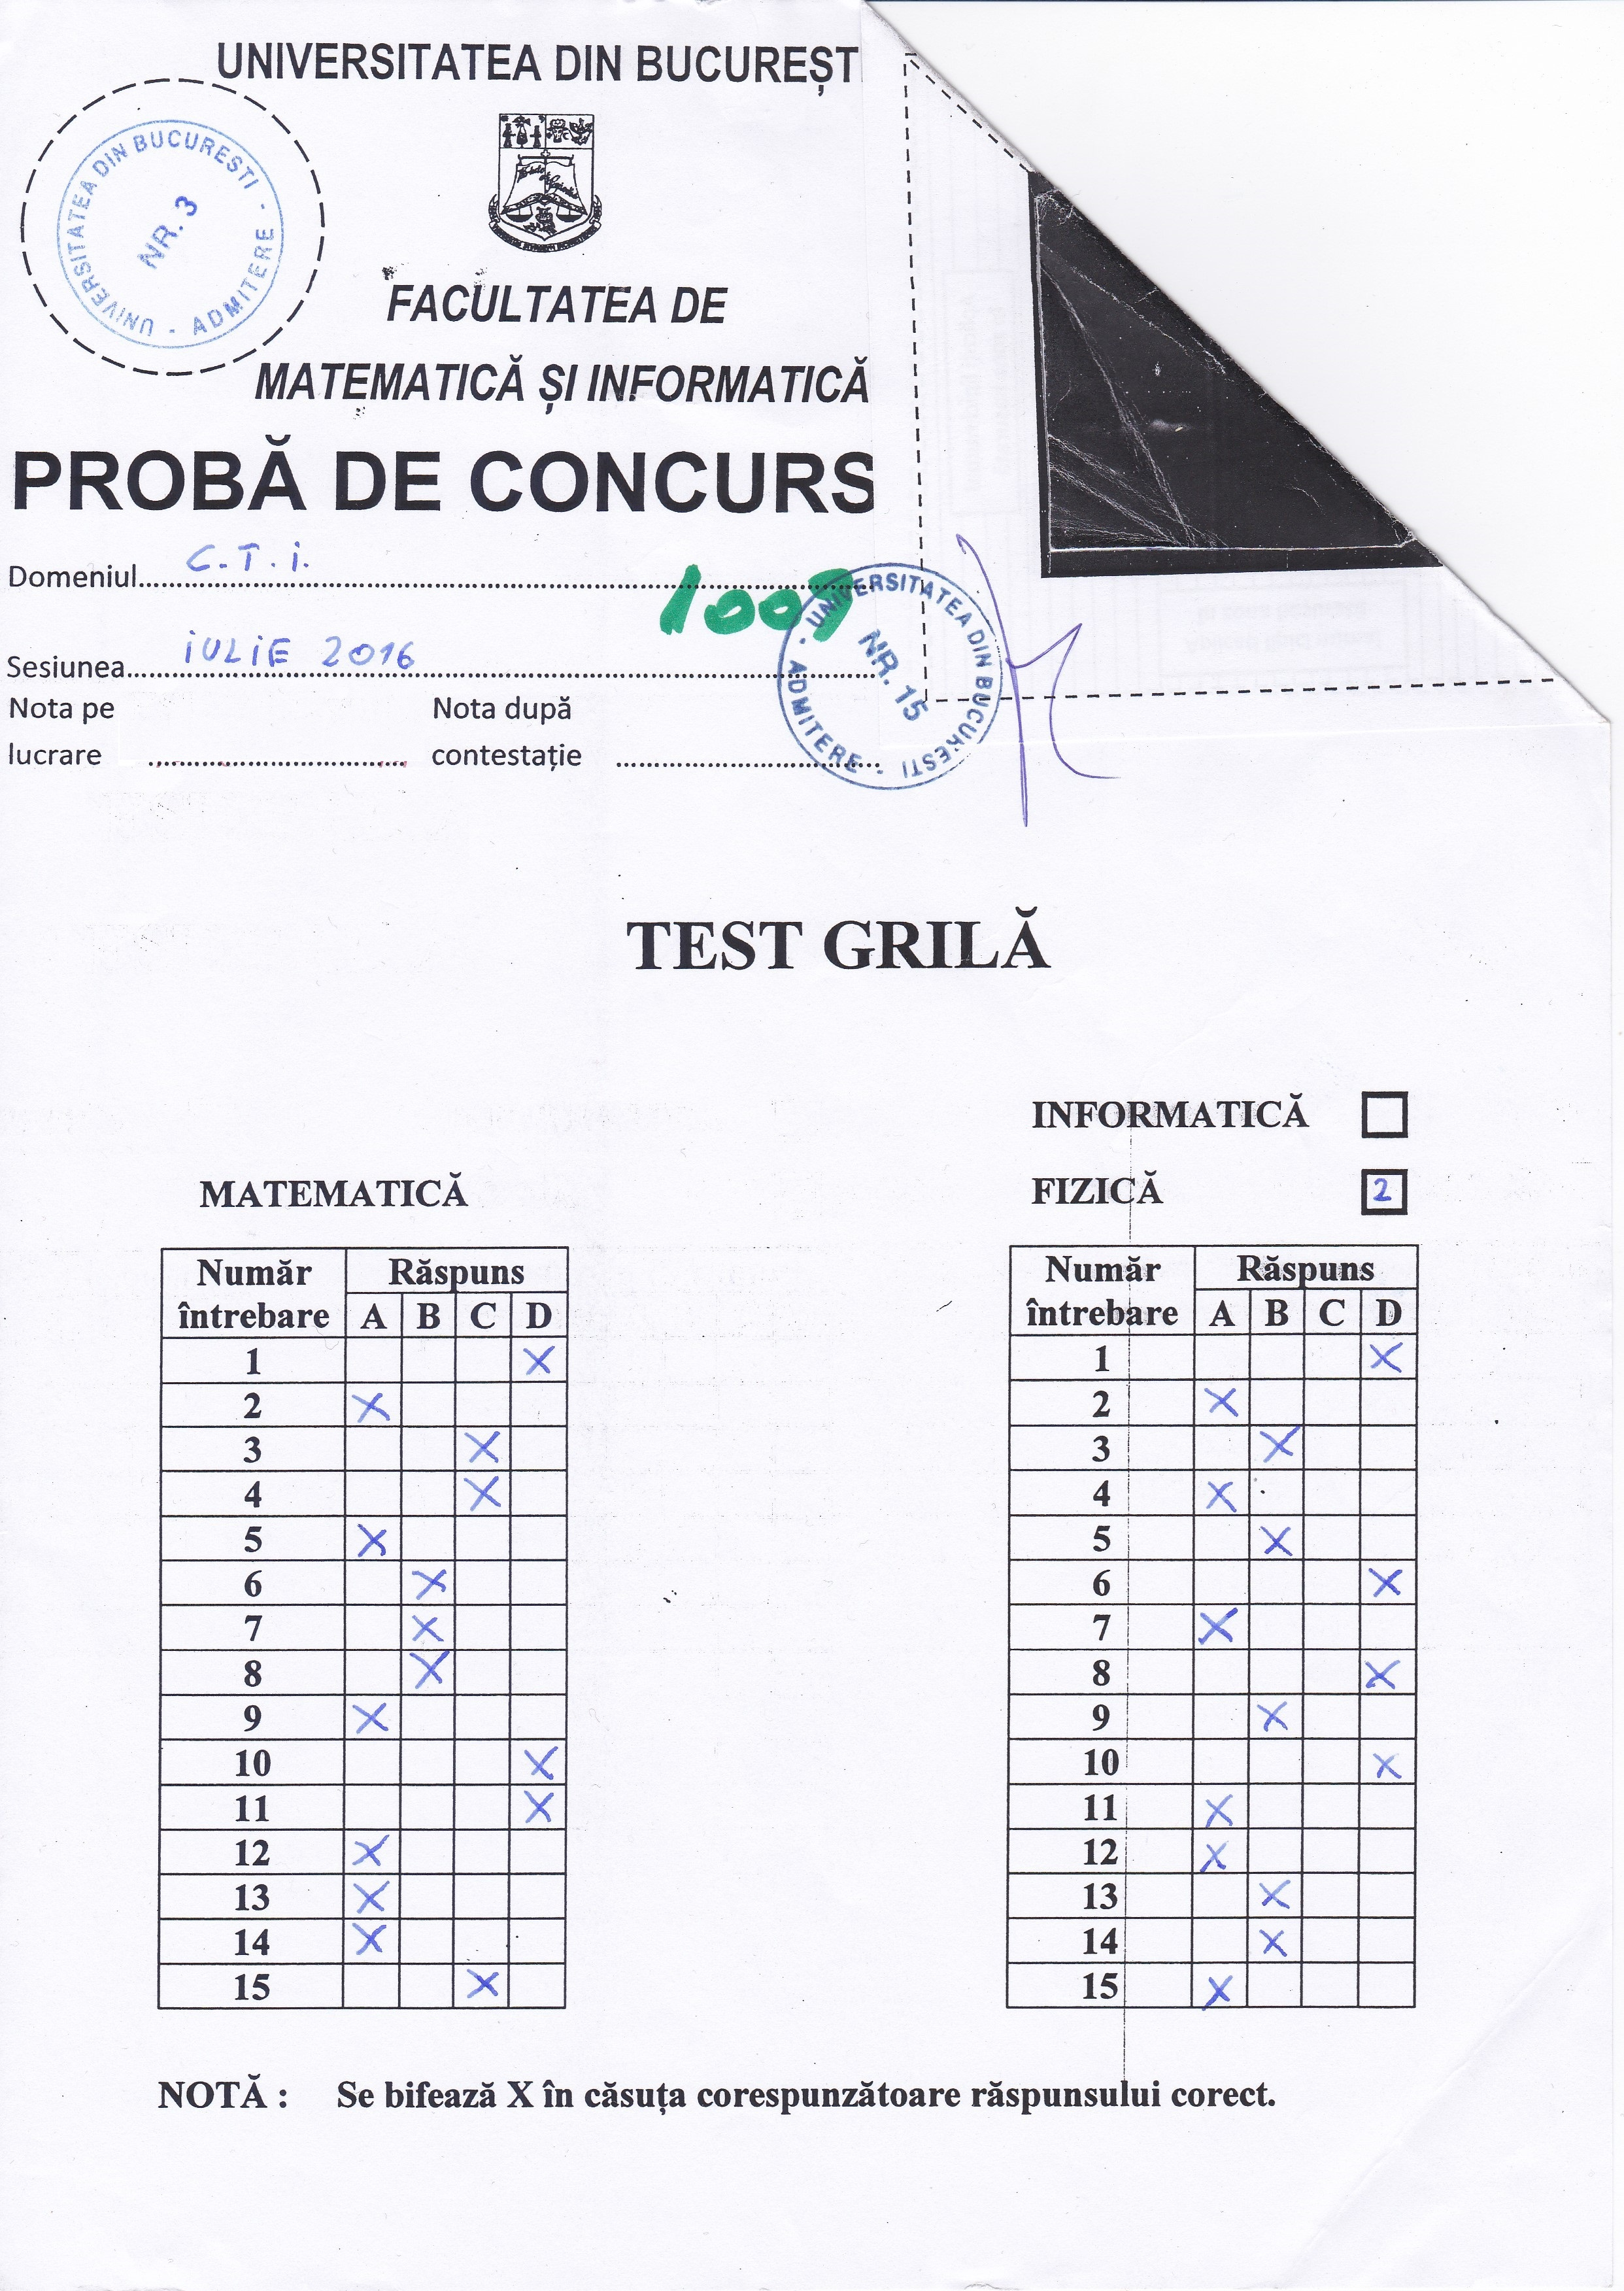
\includegraphics[width =75mm]{fig1_4} \\
		\textbf  {Figura 1.4} Lucrare completată în sesiunea iulie 2016
	\end {footnotesize} 
\end {center}
\tab Procesul actual pe care îl execută comisia de admitere în momentul corectării lucrărilor este următorul:
\begin{enumerate}
\setlength\itemsep{1pt}
\item se iau lucrările și li se atribuie un număr diferit față de cel al legitimației elevului 
\item se verifică dacă lucrarea este completată corespunzător, adică are un singur răspuns bifat pentru fiecare întrebare și numărul variantei alese este completat corect
\item primul profesor evaluator alege șablonul corespunzător variantei de subiect pe care a primit-o elevul, dar și a tipului grilei completate (informatică sau fizică)
\item se așează șablonul pe lucrarea care se corectează și se numără răspunsurile pentru fiecare dintre cele două grile din lucrare, matematică, respectiv informatică sau fizică
\item lucrarea merge la un al doilea profesor evaluator care repetă pașii 3 și 4
\item se verifică punctajele obținute de către profesori, iar dacă acestea nu corespund, lucrarea merge la un al treilea profesor pentru a fi reevaluată
\item nota finală se introduce în aplicația care centralizează rezultatele.
\end{enumerate}
\tab În urma pașilor descriși anterior rezultă faptul că timpul necesar în realizarea acestui proces este unul destul de mare. În primul rând, acest lucru este datorat faptului că trebuie analizată 
atent lucrarea pentru a nu avea mai multe răspunsuri bifate, urmând ca după să fie selectat șablonul corespunzător acesteia pentru a fi corectată. În al doilea rând, se numără răspunsurile corecte și se notează rezultatele
obținute de către primul evaluator. Pașii se reiau de către un al doilea evaluator, astfel încât timpul efectiv necesar corectării crește. În momentul în care cele două note obținute nu sunt egale, procesul se efectuează încă o dată, iar nota finală este introdusă în aplicație pentru centralizarea rezultatelor.
\\ \tab Obiectivul urmărit de către aplicația descrisă în prezenta lucrare este acela de a diminua cât mai mult activitatea factorului uman în procesul de corectare. Modalitatea de desfășurare automată a acestuia
implică atenta supraveghere a comisiei de admitere pentru a nu apărea probleme de-a lungul procesării. 
\\ \tab În cele ce urmează, facem o scurtă prezentare a procesului automat de corectare, exemplificând operațiile care se realizează asupra lucrărilor (figura 1.5).
\begin {center} 
	\begin {footnotesize} 
		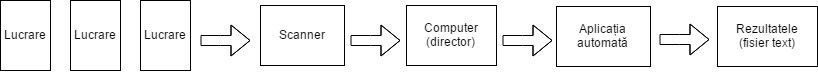
\includegraphics[width =155mm]{fig1_5} \\
		\textbf  {Figura 1.5} Schema procesului automat
	\end {footnotesize} 
\end {center}
\tab Procesul automat descris în figura 1.5 parcurge următorii pași, care vor fi detaliați în capitolele următoare:
\begin{enumerate}
\setlength\itemsep{1pt}
\item la finalul examenului de admitere lucrările se centralizează de către comisia de admitere
\item lucrările sunt scanate și imaginile digitale rezultate în urma acestui pas sunt salvate într-un director, pe mașina de calcul
\item se verifică faptul că numărul de imagini rezultate este egal cu numărul de lucrări completate
\item se introduc răspunsurile corecte în aplicație, de către comisia de admitere
\item aplicația pregătește imaginea pentru a fi corectată - se elimină zgomotul care apare în urma printării și scanării acesteia
\item se determină pozițiile la care se găsesc cele două grile în imaginea procesată la pasul curent
\item se determină răspunsurile bifate de către elev 
\item se determină tipul de grilă la care a răspuns elevul (fizică sau informatică), dar și a numărului acestei grile (1, 2, 3 sau 4)
\item se compară răspunsurile bifate de către elev cu cele introduse de către comisia de admitere
\item se determină nota finală care se bazează pe formula: Nota finală = 0.3p *  numărul răspunsurilor corecte + 1p (oficiu). 
\end{enumerate}
\tab În urma descrierii etapelor realizate de către procesul automat se observă faptul că interven-ția comisiei de admitere este una importantă în momentul scanării lucrărilor pentru a nu apărea probleme. Totodată, trebuie
ca aplicația să fie pornită, iar la sfârșitul procesării, rezultatele trebuie interpretate și analizate, pentru depistarea erorilor. Timpul efectiv de lucru al comisiei de admitere este unul redus, astfel încât existența unui program 
care să automatizeze activitatea este destul de necesară. 
\\ \tab Lucrarea de față își propune descrierea procesului automat care se realizează în momentul corectării lucrărilor. În prima parte a lucrării, reprezentată de capitolul 2, se prezintă în detaliu fundamentul teoretic care stă
la baza procesării efectuate asupra imaginilor digitale, a etapei de antrenare și testare a modelului de învățare supervizată, și anume SVM (Support Vector Machine), a descriptorului HOG (Histogram of Oriented Gradients),
a setului de date MNIST. Capitolul 3 este dedicat dezvoltării efective a aplicației prin aplicarea tehnicilor descrise în prima partea a lucrării, astfel încât se detaliază pas cu pas operațiile efectuate la fiecare etapă a procesului automat. Ultima parte a prezentei lucrări descrie rezultatele experimentale obținute în urma diverselor tehnici abordate, alături de avantajele, dezavantajele și limitările utilizării acestui program software.


\chapter*{}

\chapter {Fundamentare teoretică}
\tab Aplicația de corectare automată a testelor grilă care este descrisă în prezenta lucrare aplică principiile unui subdomeniu al inteligenței artificiale, și anume, vederea artificială. Acest subdomeniu își propune să dezvolte algoritmi și tehnici pentru mașinile de calcul, oferindu-le posibilitatea de a rezolva probleme care necesită inteligență umană. Totodată, vederea artificială este reprezentată de capacitatea unei mașini de a extrage, procesa și analiza informații din imagini, care vor fi folosite ca instrument de decizie.
\section {Detecția contururilor}
\tab În prima etapă a procesării imaginilor digitale rezultate în urma scanării se urmărește detectarea celor 8 colțuri care aparțin grilelor din pagină. Pentru a realiza acest 
pas se aplică o serie de transformări evidențiate în cele ce urmează.
\\ \tab Imaginea inițială este reprezentată în format RGB, adică este compusă din 3 canale de culoare, R-red, G-green, B-blue, astfel încât procesarea începe prin aducerea acesteia la un format greyscale (în tonuri de gri).  
Pentru a obține o imagine în tonuri de gri, fiecare pixel rezultat va avea o valoare calculată după formula următoare: $x=0.299*r+0.587*g+0.114*b$, unde r, g, b sunt intensitățile fiecărui canal aparținând imaginii color, iar x este valoarea 
rezultată care este atribuită pixelului din imaginea în tonuri de gri\cite{book1}.
\\ \tab Asupra imaginii în tonuri de gri se aplică un filtru Gaussian de blurare\cite{book2}, utilizat în aplicațiile de vedere artificială pentru reducerea zgomotului și eliminarea detaliilor. Filtrul este reprezentat sub forma unei matrice pătratice de dimensiune n,
unde n este un număr impar. În figura 2.1 este prezentat un astfel de filtru de blurare, de dimensiune 3. 
\begin {center} 
	\begin {footnotesize} 
		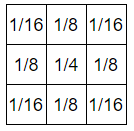
\includegraphics[width =33mm]{fig2_1} \\
		\textbf  {Figura 2.1} Filtru Gaussian de blurare de dimensiune $3\times3$
	\end {footnotesize} 
\end {center}
\tab Detectarea muchiilor din imagine este, de asemenea, o tehnică folosită în vederea obținerii celor 8 colțuri care aparțin grilelor, fiind realizată cu ajutorul detectorului Canny. Asupra imaginii blurate se aplică două măști convoluționale
reprezentate sub forma unor matrice $3\times3$ (figura 2.2). Prin structura lor, aceste filtre convoluționale calculează derivatele parțiale în direcțiile x și y ale imaginii, rezultând astfel valoarea gradientului pentru fiecare pixel al imaginii.
\begin {center} 
	\begin {footnotesize} 
		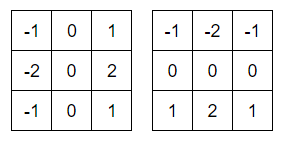
\includegraphics[width = 67mm]{fig2_2}\\
		\textbf  {Figura 2.2} Filtre convoluționale-derivatele parțiale în direcțiile x și y
	\end {footnotesize} 
\end {center}
\tab În urma aplicării filtrelor convoluționale asupra unei imagini se obțin rezultatele din figura 2.3, unde prima imagine este cea inițială, cea de-a doua este imaginea pentru care s-a aplicat filtrul convoluțional cu derivata parțială în direcția x,
iar cea de-a treia este imaginea pentru care s-a aplicat filtrul convoluțional cu derivata parțială în direcția y.
\begin {center} 
	\begin {footnotesize} 
		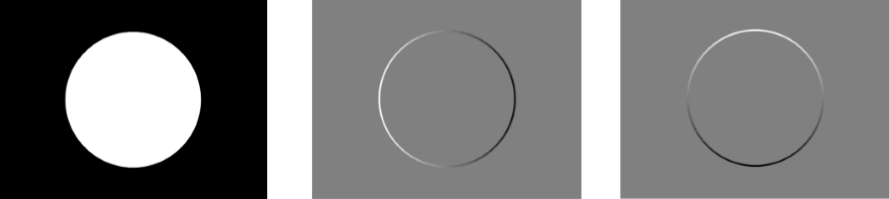
\includegraphics[width = 130mm]{fig2_3} \\
		\textbf  {Figura 2.3} Rezultatele aplicării filtrelor convoluționale
	\end {footnotesize} 
\end {center}
\tab Determinarea valorilor gradientului, a magnitudinii gradientului și a direcției acestuia sunt realizate folosind următoarele formule de calcul ( $f:\mathbb{R}^2\rightarrow \mathbb{R}$,  $f(x,y)$ = intensitatea imaginii la x, y): 
	\[\nabla f =  \Bigl[\frac{\partial f}{\partial x}, \frac{\partial f}{\partial y}\Bigr] \tab
	\|\nabla f\| =  \sqrt {\big( \frac{\partial f}{\partial x}\big)^2 + \big(\frac{\partial f}{\partial y}\big)^2} \tab
	\theta = \arctan\big(  \frac{\partial f}{\partial x} /  \frac{\partial f}{\partial y}\big)\]
\tab În figura 2.4 se prezintă imaginea rezultată în urma calculării magnitudinii gradientului (în partea dreaptă) pentru imaginea inițială (în partea stângă):
\begin {center} 
	\begin {footnotesize} 
		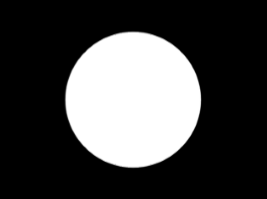
\includegraphics[width = 40mm]{fig2_4_1}
		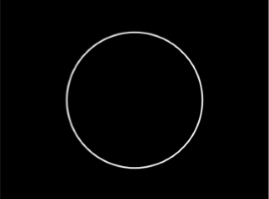
\includegraphics[width = 40mm]{fig2_4_2} \\
		\textbf  {Figura 2.4} Calcularea magnitudinii gradientului
	\end {footnotesize} 
\end {center}
\tab În continuarea procesului de detectare a muchiilor, imaginii rezultate în urma calculării magnitudinii gradientului și a orientării acestuia i se aplică metoda eliminării non-maximelor. Această metodă constă 
în parcurgerea a două etape: compararea magnitudinii gradienților pixelului curent de pe o anumită muchie în direcțiile valorilor pozitive și negative ale gradientului determinat. Dacă valoarea calculată este cea mai mare comparativ cu cea a restul pixelilor din imagine care au aceeași orientare, înseamnă că acest pixel aparține muchiei, altfel este eliminat, pentru că nu aparține muchiei. 
\\ \tab Metoda de detectare a muchiilor implică existența unor praguri de valori, unul inferior, respectiv unul superior în funcție de care se formează imaginea finală (așa numita metodă de Hysteresis). Prin urmare, ultimul pas în detectarea muchiilor este
reprezentat de realizarea unor operații de comparare pentru determinarea rezultatului final, după cum urmează:
\begin{itemize}
\setlength\itemsep{1pt}
\item dacă gradientul unui pixel este mai mare decât pragul superior, acesta este acceptat ca aparținând unei muchii
\item dacă gradientul unui pixel este mai mic decât pragul inferior, acesta este eliminat
\item dacă gradientul unui pixel se află între cele două valori de prag, acesta este acceptat numai dacă este conectat cu un pixel al cărui gradient are o valoare mai mare decât pragul superior.
\end{itemize}
\tab În figura 2.5 se observă răspunsul metodei de detectare a muchiilor asupra unei imagini inițiale (imaginea din partea stângă), căreia i s-a aplicat prima dată valorile de prag inferior=0, respectiv superior=50 (imaginea din mijloc), iar 
a doua oară valorile de prag inferior=205, respectiv prag superior=255 (imaginea din partea dreaptă). În momentul în care se aleg valori mici pentru pragul inferior, respectiv pragul superior, gradienții calculați pentru pixelii din imagine depășesc aceste praguri, ceea
ce face ca respectivii pixeli să fie atașați unei anumite muchii. Pe de altă parte, dacă valorile de prag inferior și superior sunt mari, pixelii cu gradient mic sunt eliminați, astfel încât în imaginea rezultată vor fi afișate doar muchiile cele mai importante. 
\begin {center} 
	\begin {footnotesize} 
		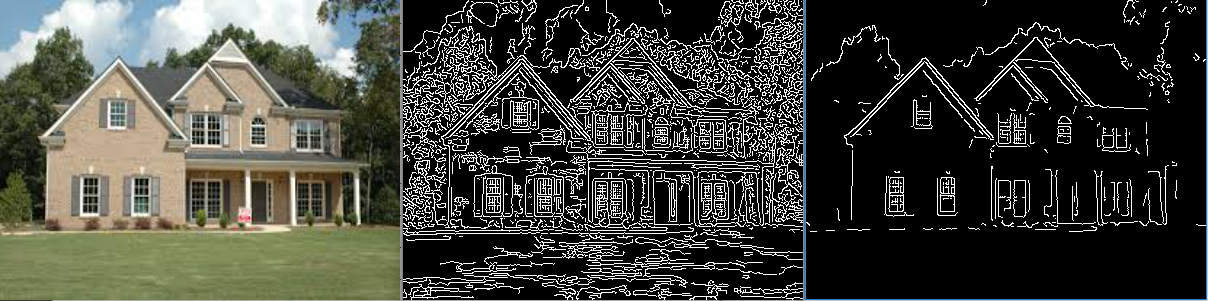
\includegraphics[width = 160mm]{fig2_5} \\
		\textbf  {Figura 2.5} Detectarea muchiilor
	\end {footnotesize} 
\end {center}
\tab Detecția muchiilor folosind Canny reprezintă etapa inițială pentru procesul de găsire a contururilor obiectelor dintr-o imagine. Problema care apare în momentul detectării este reprezentată de zgomotul care a fost eliminat, sau de calitatea slabă a imaginii, astfel încât muchiile
rezultate nu reprezintă contururi închise. Pentru închiderea acestora în vederea acurateții procesului de detectare a lor, asupra imaginii se aplică o transformare morfologică. Există mai multe tipuri de transformări care se pot folosi, însă cea necesară 
pentru detectarea contururilor grilelor este cea de închidere. Pentru realizarea procesului se definește un nucleu, reprezentat sub forma unei matrice pătratice, de dimensiune n, unde n este un număr impar, în funcție de care se realizează transformarea.
 În figura 2.6 se aplică operația de închidere a muchiilor pentru imaginea inițială din partea stângă, rezultatul fiind imaginea din partea dreaptă.   
\begin {center} 
	\begin {footnotesize} 
		
\includegraphics[width = 60mm]{fig2_6} \\
		\textbf  {Figura 2.6} Transformarea morfologică\\ de închidere \cite{opencv1}
	\end {footnotesize} 
\end {center}
\tab În figura 2.7 se evidențiază răspunsul aplicării transformării morfologice de închidere a muchiilor pentru imaginea în care s-au detectat muchiile cu valorile de prag 205, respectiv 255. În primă fază, s-a aplicat operația de închidere cu un nucleu de dimensiune 3,
în care toate elementele aveau valoarea 1, iar în a două fază s-a aplicat operația cu un nucleu de dimensiune 7.
\begin {center} 
	\begin {footnotesize} 
		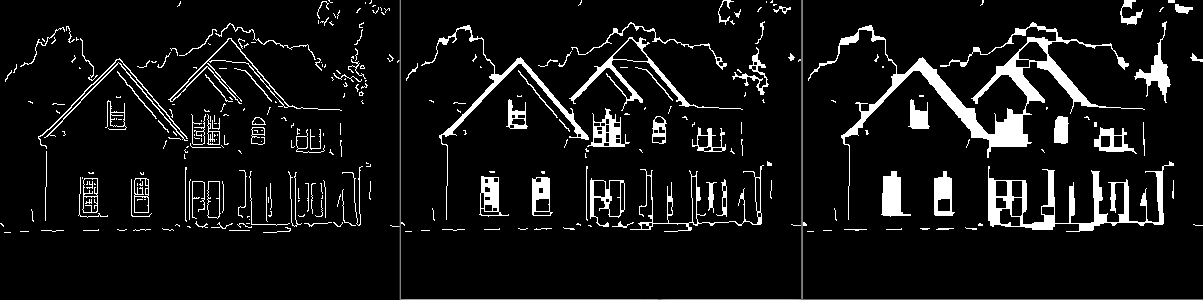
\includegraphics[width = 160mm]{fig2_7} \\
		\textbf  {Figura 2.7} Transformarea morfologică de închidere
	\end {footnotesize} 
\end {center}
\tab Detecția contururilor se realizează folosind o metodă care primește ca parametru imaginea pentru care s-au detectat muchiile, folosind în acest caz detectorul Canny. Există mai multe moduri de selecție a contururilor, printre care, RETR\textunderscore EXTERNAL
(doar contururile exterioare) sau RETR\textunderscore LIST (toate contururile). De asemenea, metoda de determinare a contururilor primește ca parametru și o funcție de aproximare, spre exemplu CHAIN\textunderscore APPROX\textunderscore SIMPLE, unde rezultatul este reprezentat doar de valorile coordonatelor capetelor segmentelor care compun un anumit obiect existent în imagine, în comparație cu CHAIN\textunderscore APPROX\textunderscore NONE, unde rezultatul este reprezentat de toate punctele care aparțin conturului. 
\\ \tabÎn figura 2.8 se afișează rezultatele funcției CHAIN\textunderscore APPROX\textunderscore NONE (în stânga), reprezentată de toate punctele $(x,y)$, comparativ cu funcția CHAIN\textunderscore APPROX\textunderscore SIMPLE (în dreapta) reprezentată de cele 4 colțuri $(x,y)$ ale conturului.
\begin {center} 
	\begin {footnotesize} 
		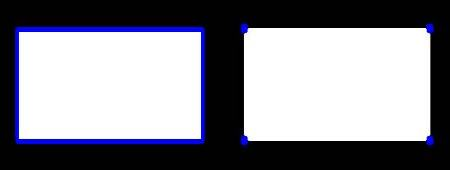
\includegraphics[width = 100mm]{fig2_8} \\
		\textbf  {Figura 2.8} Detecția contururilor\cite{opencv2}
	\end {footnotesize} 
\end {center}
\tab Lista de contururi obținută prin aplicarea metodei descrise mai sus se aproximează folosind o funcție care aplică algoritmul Ramer-Douglas-Peucker\cite{wikip1}. Ideea algoritmului constă în următorii pași: pentru o curbă formată din mai multe segmente de dreaptă se poate găsi o aproximare reprezentată de o curbă similară cu mai puține puncte.  În realizarea algoritmului se definește diferența bazată pe distanța maximă dintre curba inițială și cea rezultată, diferență care poartă numele de distanța Hausdorff dintre curbe. Rezultatul aplicării metodei descrise asupra unei curbe este prezentat în figura 2.9 (cu roșu este reprezentată curba inițială, iar cu albastru curba rezultată).
\begin {center} 
	\begin {footnotesize} 
		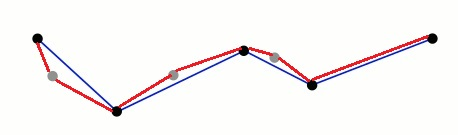
\includegraphics[width = 130mm]{fig2_9} \\
		\textbf  {Figura 2.9} Aplicarea algoritmului Ramer-Douglas-Peucker
	\end {footnotesize} 
\end {center}
\section{Etapa de antrenare}
\tab În aplicația descrisă în prezenta lucrare este necesară existența unui clasificator al cărui scop este acela de recunoaștere a unei cifre scrise de mână, care reprezintă numărul variantei de subiect rezolvată într-o anumită lucrare. În acest sens, prezentăm în cele ce urmează descriptorul histogramelor de gradienți orientați (HOG), clasificatorul Support Vector Machine (SVM), setul de date MNIST și metoda de învățare supervizată.
\subsection {HOG}
\tab În vederea antrenării și testării clasificatorului, o etapă preliminară este reprezentată de extragerea caracteristicilor seturilor de date. O metodă este aceea a histogramelor de gradienți orientați (HOG)\cite{opencv3} pentru anumite puncte dintr-o imagine. 
Pentru a determina aceste puncte se aplică peste imaginea inițială un caroiaj, reprezentat de o structură de drepte verticale și orizontale, a cărui dimensiune este specificată la începutul procesului. 
\\ \tab Algoritmul de calculare a histogramelor este efectuat în 5 pași, după cum urmează:
\begin{enumerate}
\setlength\itemsep{1pt}
\item normalizarea imaginii, care poate fi un pas opțional - rolul acestui pas este de a reduce efectele de iluminare ale imaginii
\item determinarea valorii gradientului imaginii în direcțiile x și y - se evidențiază conturul obiectelor din imagine, dar și textura existentă
\item determinarea histogramelor de gradienți - pentru fiecare celulă din imagine se calculează o histogramă locală de gradient și, totodată, se determină orientarea pixelilor 
\item normalizarea între blocurile care au rezultat în urma aplicării caroiajului - implică faptul că rezultatele nu sunt influențate de metodele de iluminare, de umbrire și de evidențiere a muchiilor 
\item determinarea vectorului de caracteristici în care sunt salvate valorile histogramelor calculate.
\end{enumerate}
\tab Pasul 3 este reprezentat de o succesiune de operații în care dimensiunea descriptorului HOG este dată de numărul de celule existente și numărul de orientări ale unui gradient. Obținerea descriptorului HOG se realizează astfel:
\begin{itemize}
\setlength\itemsep{1pt}
\item pentru fiecare dintre punctele care aparțin matricei caroiajului realizat asupra imaginii se generează ferestre centrate în respectivele puncte, care la rândul lor sunt împărțite din nou în alte celule (fiecare celulă este reprezentată de o matrice pătratică de dimensiune n)
\item pentru celulele nou definite se calculează histogramele aferente lor, având dimensiunea dată de numărul orientărilor pixelilor
\item în final, se concatenează histogramele obținute (în total sunt $x^2*y$ histograme, unde $x$=numărul de celule creat la pasul anterior, iar $y$=numărul de celule existent în caroiajul creat inițial).
\end{itemize}
\tab În figura 2.10 se evidențiază calculul histogramei de gradienți orientați pentru matricele aferente direcției gradientului, respectiv magnitudinii acestuia. Pentru prima pereche valoarea direcției gradientului este 80, iar magnitudinea este 2, astfel încât în HOG va exista perechea (80, 2). Pentru o valoare egală cu 10 a direcției gradientului, care este la jumătatea distanței dintre 0 și 20, se generează perechile (0, 2) și (20, 2).
\begin {center} 
	\begin {footnotesize} 
		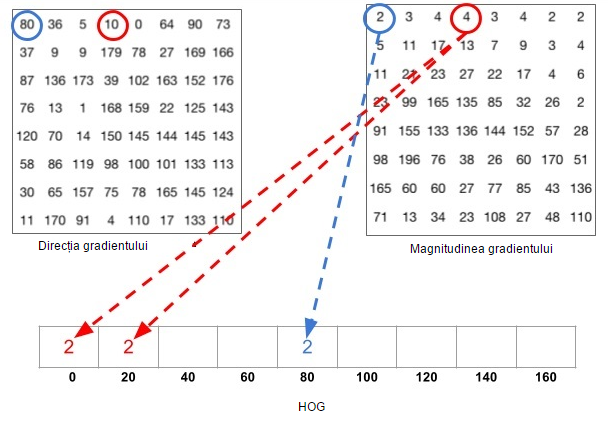
\includegraphics[width = 135mm]{fig2_10} \\
		\textbf  {Figura 2.10} Calcularea HOG
	\end {footnotesize} 
\end {center}
\tab În figura 2.11 este reprezentat întregul proces de calculare a descriptorului HOG pentru o imagine.
\begin {center} 
	\begin {footnotesize} 
		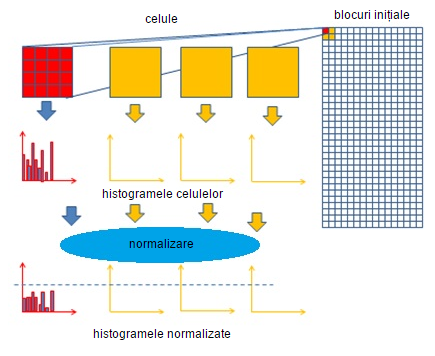
\includegraphics[width = 120mm]{fig2_11} \\
		\textbf  {Figura 2.11} Calcularea descriptorului HOG\cite{opencv4}
	\end {footnotesize} 
\end {center}
\tab În figura 2.12 este prezentată imaginea inițială pentru care s-au calculat histogramele de gradienți orietentați:
\begin {center} 
	\begin {footnotesize} 
		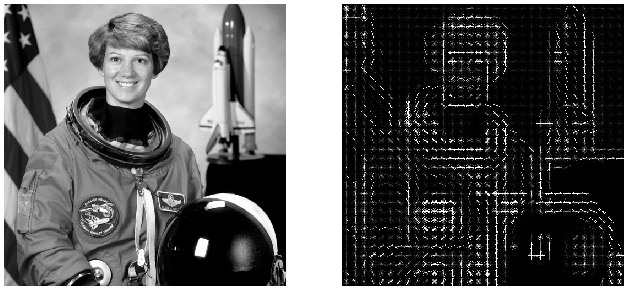
\includegraphics[width = 120mm]{fig2_12} \\
		\textbf  {Figura 2.12} Rezultatul calculării descriptorului HOG\cite{opencv5}
	\end {footnotesize} 
\end {center}

\subsection{SVM}
\tab Support Vector Machine\cite{wikip2, wikip3, sklearn} reprezintă un clasificator al cărui rol este acela de a face o distincție sau o deosebire între două sau mai multe categorii de obiecte. Ideea principală a clasificatorului constă în faptul că pentru un set de date de antrenare (imagini și etichetele lor), prin tehnica învățării supervizate se pot prezice etichetele pentru noi imagini de test.
\\ \tab Clasificarea datelor este o problemă de actualitate în domeniul machine learning-ului (după definiția lui Arthur Samuel din 1959, machine learning-ul reprezintă ``abilitatea mașinilor de calcul de a învăța și reproduce o anumită funcționalitate
fară a fi programată în acest sens``). Să presupunem ca date de antrenare niște puncte ce aparțin uneia dintre cele două clase (puncte roșii sau verzi). Scopul clasificării este reprezentat de decizia apartenenței unui nou punct la una dintre cele două clase. Pentru expunerea ideii principale se va considera un plan 2D, iar hiperplanul separator pentru cele două clase existente va fi o linie dreaptă. În figura 2.13, dreapta h1 nu se separă clasele, dreapta h2 separă clasele cu un mic factor de eroare, iar dreapta h3 separă clasele fără eroare.
\begin {center} 
	\begin {footnotesize} 
		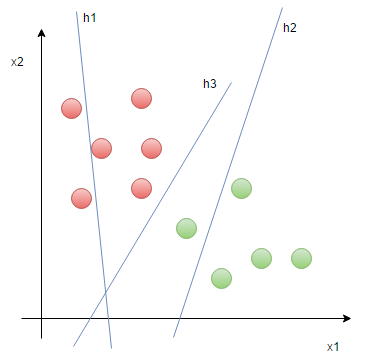
\includegraphics[width = 90mm]{fig2_13} \\
		\textbf  {Figura 2.13} Separarea claselor de obiecte
	\end {footnotesize} 
\end {center}
\tab În cazul acestui clasificator, orice punct este văzut ca un vector p-dimensional, iar scopul este de a găsi un hiperplan de dimensiune (p-1) care să separe punctele date. Orice hiperplan este scris sub forma unui set de puncte $\vec{x}$, unde $\vec{x}$ se mai numește și vector suport, care indeplinește condiția:
$\vec{w}\cdot \vec{x} - b = 0, \vec{w}$ este vectorul normal la hiperplan, iar valoarea $\frac{b}{\|\vec{w}\|}$ determină valoarea de deplasare a hiperplanului raportată  la origine și în direcția vectorului $\vec{w}$. În figura 2.14 sunt reprezentate 3 hiperplanuri, dintre care 
cel din mijloc nu are eroare, iar celelalte două au erori minime pentru un clasificator antrenat cu eșantioanele prezentate. 
\begin {center} 
	\begin {footnotesize} 
		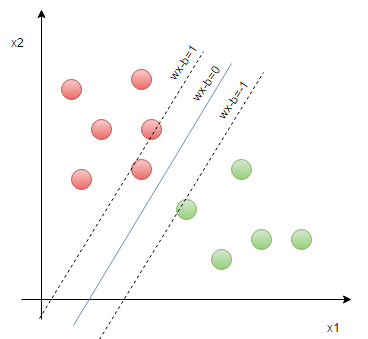
\includegraphics[width = 90mm]{fig2_14} \\
		\textbf  {Figura 2.14} Determinarea hiperplanurilor
	\end {footnotesize} 
\end {center}


\subsection{MNIST}
\tab MNIST (Modified National Institute of Standards and Technology database) \cite{mnist1} reprezintă un set de date utilizat în aplicațiile de vedere artificială, format din imagini cu cifre scrise de mână a căror dimensiune este de $28\times28$ pixeli (figura 2.15). 
Acest set de date cuprinde 60.000 de imagini de antrenare și 10.000 de date de test. 
\begin {center} 
	\begin {footnotesize} 
		
\includegraphics[width = 90mm]{fig2_15} \\
		\textbf  {Figura 2.15} Imagini din setul MNIST
	\end {footnotesize} 
\end {center}
\tab Alături de setul de imagini se definește și un set de etichete care reprezintă valoarea cifrei pentru o anumită imagine. Pentru datele din figura 2.15 etichetele sunt 5, 0, 4, 1. Fiecare imagine este stocată sub forma unei matrice de dimensiune $28\times28$ pixeli, ca în exemplul din figura 2.16.
\begin {center} 
	\begin {footnotesize} 
		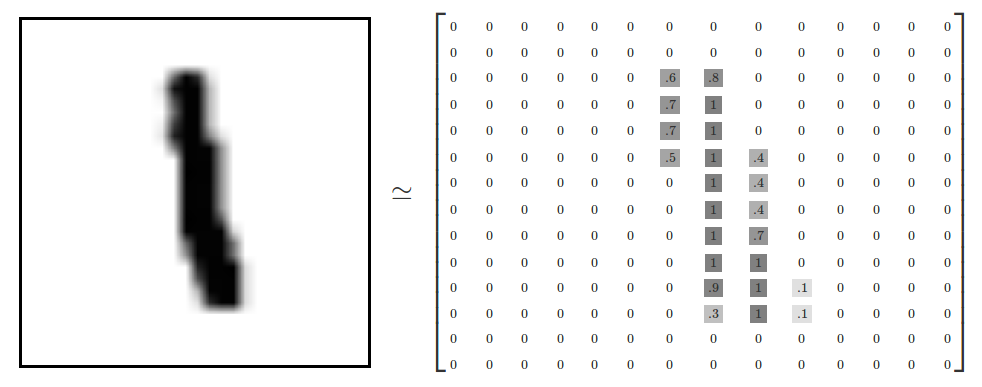
\includegraphics[width = 80mm]{fig2_16} \\
		\textbf  {Figura 2.16} Matricea unei cifre din setul MNIST
	\end {footnotesize} 
\end {center}
\tab De-a lungul timpului s-au scris mai multe lucrări științifice în încercarea de a obține o eroare cât mai mică în momentul antrenării clasificatorilor pentru recunoașterea cifrelor scrise de mână. O lucrare în care a fost abordat principiul rețelelor neuronale convoluționale a reușit să scadă procentul erorii la o valoare de 0.23\%. De asemenea, creatorii setului de date MNIST au reușit folosind clasificatorul SVM să obțină o eroare de 0.8\%.  
\subsection{Învățarea supervizată}
\tab Tehnica învățării supervizate\cite{wikip4} se aplică în majoritatea aplicațiilor de machine learning. Această metodă este descrisă prin crearea unei funcții de predicție, antrenată pentru un set de date de intrare și un set de etichete. Scopul clasificatorului este acela de a determina eticheta unei imagini care aparține unui set de date de testare. 
\\ \tab În momentul realizării modelului se parcurg datele de intrare (imaginile) și datele de ieșire (etichetele) în paralel. Iterativ, se fac predicții între aceste perechi de date, iar procesul de învățare supervizată se încheie atunci când algoritmul atinge un nivel de acuratețe ridicat (valoarea indică raportul dintre numărul de imagini care au fost detectate corect și numărul total de imagini pentru care s-a testat modelul). 
\\ \tab Există două tipuri de învățare supervizată, și anume clasificarea și regresia. Clasificarea este realizată în momentul în care datele de ieșire pot fi împărțite în mai multe categorii (cifre de 0, 1, 2 și 3 sau puncte roșii și verzi). Regresia se folosește atunci când datele de ieșire au ca rezultat o valoare reală (lățime sau greutate). Tehnica învățării supervizate, formată din procesul de învățare și cel de testare, este prezentată în figura 2.17.
\begin {center} 
	\begin {footnotesize} 
		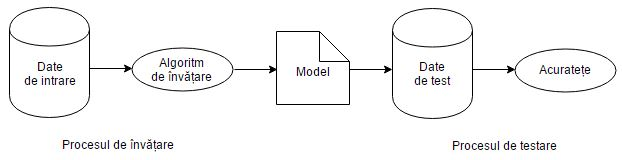
\includegraphics[width = 155mm]{fig2_17} \\
		\textbf  {Figura 2.17} Tehnica învățării supervizate
	\end {footnotesize} 
\end {center}
\tab În aplicația descrisă în prezenta lucrare procesul de învățare se realizează folosind clasificatorul SVM, descriptorul HOG, iar setul de date de antrenare și testare este MNIST. 

\chapter*{}

\chapter{Dezvoltarea aplicației}
\tab Aplicația descrisă în prezenta lucrare a fost dezvoltată pe mai multe module, care urmează a fi detaliate în capitolul de față, și anume:
\begin{enumerate}
\setlength\itemsep{1pt}
\item extragerea grilelor din lucrare
\item determinarea răspunsurilor bifate de către elev 
\item determinarea tipului de grilă la care elevul a răspuns (fizică sau informatică), dar și a numărului variantei primite (1, 2, 3 sau 4)
\item compararea răspunsurilor bifate de către elev cu cele introduse de către comisia de admitere
\item determinarea notei finale care se bazează pe formula: Nota finală = 0.3p *  numărul răspunsurilor corecte + 1p (oficiu) și scrierea rezultatelor într-un fișier text
\item testarea funcționalităților implementate
\item realizarea interfeței cu utilizatorul.
\end{enumerate}
\section{Extragerea grilelor din lucrare}
\tab Prima etapă efectuată în vederea extragerii grilelor este reprezentată de eliminarea zgomotului din imaginile digitale. În urma printării și scanării lucrărilor apariția zgomotului este inevitabilă, iar pentru o detectare corectă a elementelor importante dintr-o imagine, acest zgomot trebuie eliminat. În figura 3.1 sunt reprezentate diverse tipuri de zgomot care pot apărea în imaginile digitale.
\begin {center} 
	\begin {footnotesize} 
		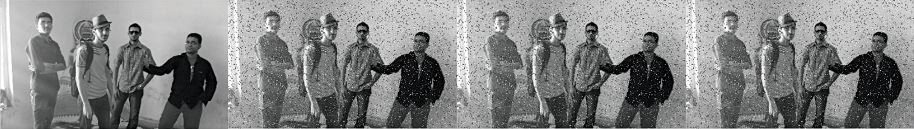
\includegraphics[width = 160mm]{fig3_1} \\
		\textbf  {Figura 3.1} Tipuri de zgomot \\ 1. Imaginea originală \hspace{11mm} 2. Zgomot ``pistrui``  \hspace{10mm} 3. Zgomot Gaussian \hspace{10mm} 4. Zgomot ``sare și piper``
	\end {footnotesize} 
\end {center}
\tab Metoda de eliminare constă dintr-o serie de transformări, care sunt aplicate fiecărei lucrări în format digital. Inițial, imaginea este transformată din RGB în tonuri de gri și acesteia i se aplică un filtru de blurare, al cărui rol este acela de eliminare a detaliilor. Pixelii din imagine care formează zgomotul au o intensitate mare, astfel încât se definește o valoare de prag în funcție de care se va realiza eliminarea.
\\ \tab În acest context, procesarea este realizată după cum urmează: pixelii cu o intensitate sub valoarea pragului formează obiecte importante din imaginea digitală, intensitatea lor devenind 0 (pixeli negri), iar cei cu o valoare peste cea a pragului, reprezintă zgomot și vor fi eliminați, devenind 255 (pixeli albi). În figura 3.2 sunt reprezentate în stânga imaginea inițială, iar în dreapta imaginea rezultată în urma eliminării zgomotului, folosind un prag cu valoarea de 180 (pentru detalierea aspectelor de implementare se va decupa din imaginea digitală partea de sus pentru care nu vom efectua nicio procesare).
\begin {center} 
	\begin {footnotesize} 
		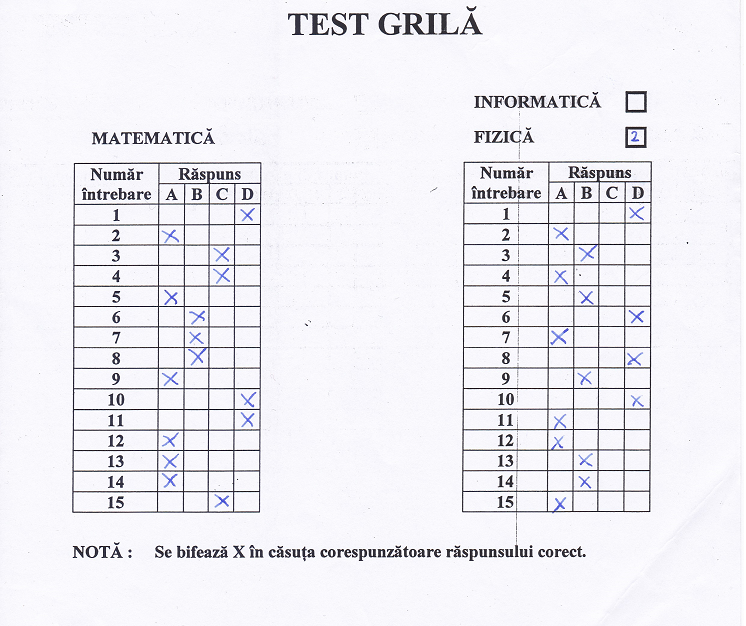
\includegraphics[width = 73mm]{fig3_2_1} 
		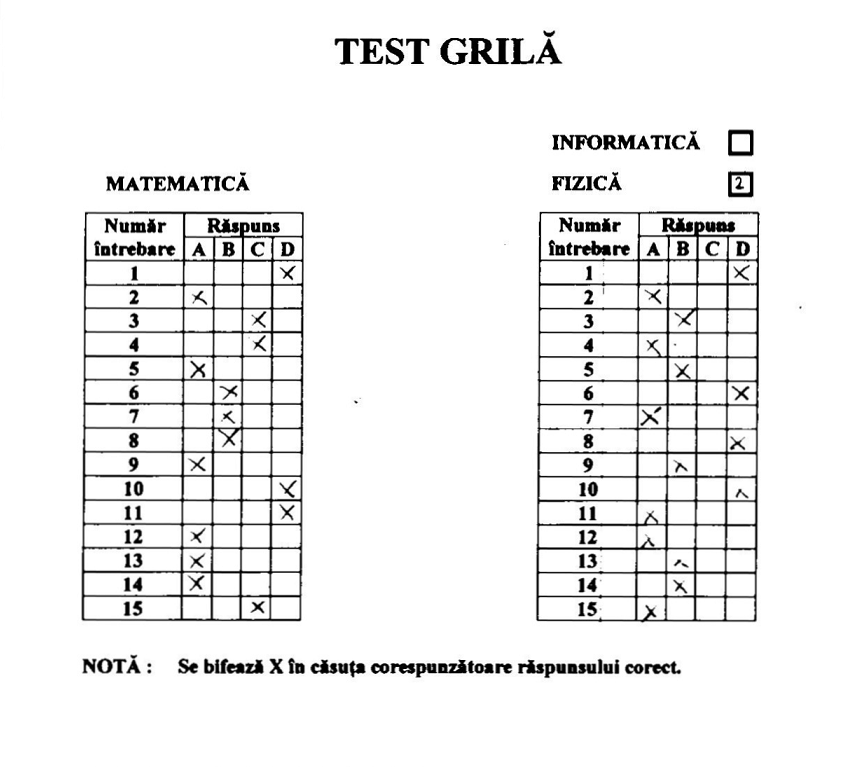
\includegraphics[width = 73mm]{fig3_2_2} \\
		\textbf  {Figura 3.2} Eliminarea zgomotului cu o valoare de prag de 180 
	\end {footnotesize} 
\end {center}
\tab În urma eliminării zgomotului din imaginea digitală, procesul de extragere a grilelor continuă cu blurarea imaginii folosind un filtru Gaussian de dimensiune 3. Rolul acestui pas este acela de eliminare a detaliilor din imaginea fără zgomot, astfel încât detecția muchiilor care urmează a fi efectuată în continuare să ofere ca răspuns doar muchiile importante (cele care aparțin efectiv grilelor). În figura 3.3 este evidențiat răspunsul filtrului Gaussian asupra imaginii din stânga, de dimensiune 5, respectiv 15.
\begin {center} 
	\begin {footnotesize} 
		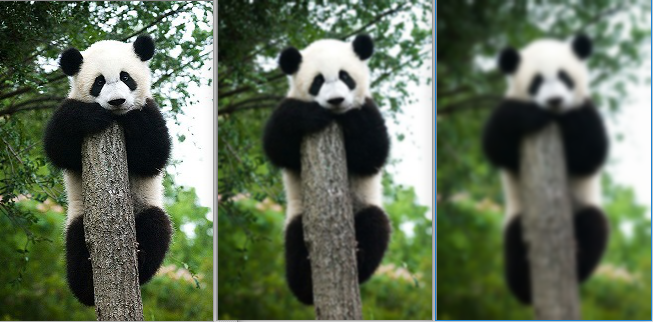
\includegraphics[width = 110mm]{fig3_3}\\
		\textbf  {Figura 3.3} Răspunsul filtrului Gaussian de dimensiune 5, respectiv 15 
	\end {footnotesize} 
\end {center}
\tab Detecția de muchii în imaginea blurată constituie un proces al cărui răspuns reprezintă formatul asupra căruia se aplică metoda de extragere a contururilor obiectelor. Acest pas este realizat folosind detectorul Canny, alături de valorile de prag inferior și prag superior. În vederea detecției muchiilor care fac parte din grilele existente în imagine se folosesc valorile de prag 10, respectiv 250. În figura 3.4 este reprezentat rezultatul detecției muchiilor care a fost efectuată conform detaliilor specificate.
\begin {center} 
	\begin {footnotesize} 
		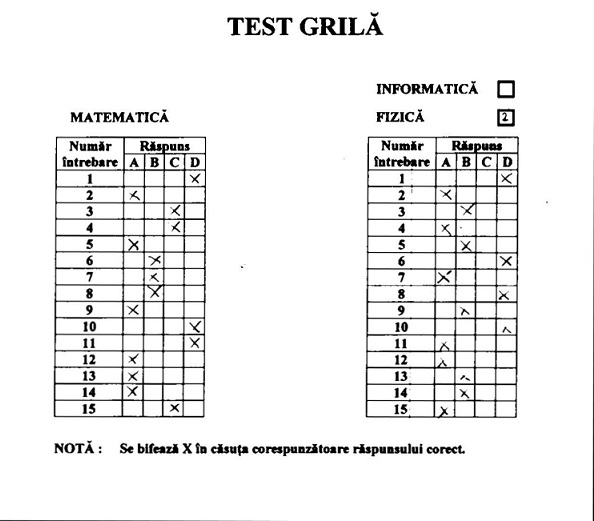
\includegraphics[width = 73mm]{fig3_4_1} 
		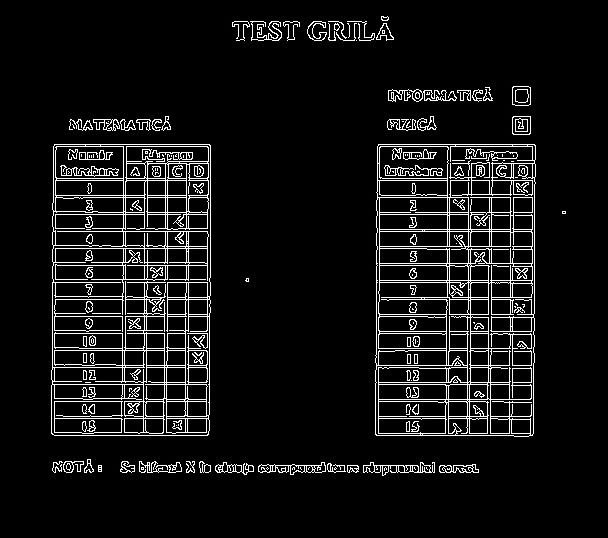
\includegraphics[width = 73mm]{fig3_4_2} \\
		\textbf  {Figura 3.4} Detecția muchiilor folosind Canny (imagine cu filtrul Gaussian)
	\end {footnotesize} 
\end {center}
\tab În figura 3.5 este evidențiat răspunsul detectorului de muchii aplicat peste imaginea din care s-a eliminat zgomotul, dar care nu a fost blurată folosind filtrul Gaussian. Rezultatul constă în găsirea de muchii pentru zone în care există detalii, astfel încât procesarea nu oferă un răspuns adecvat.
\begin {center} 
	\begin {footnotesize} 
		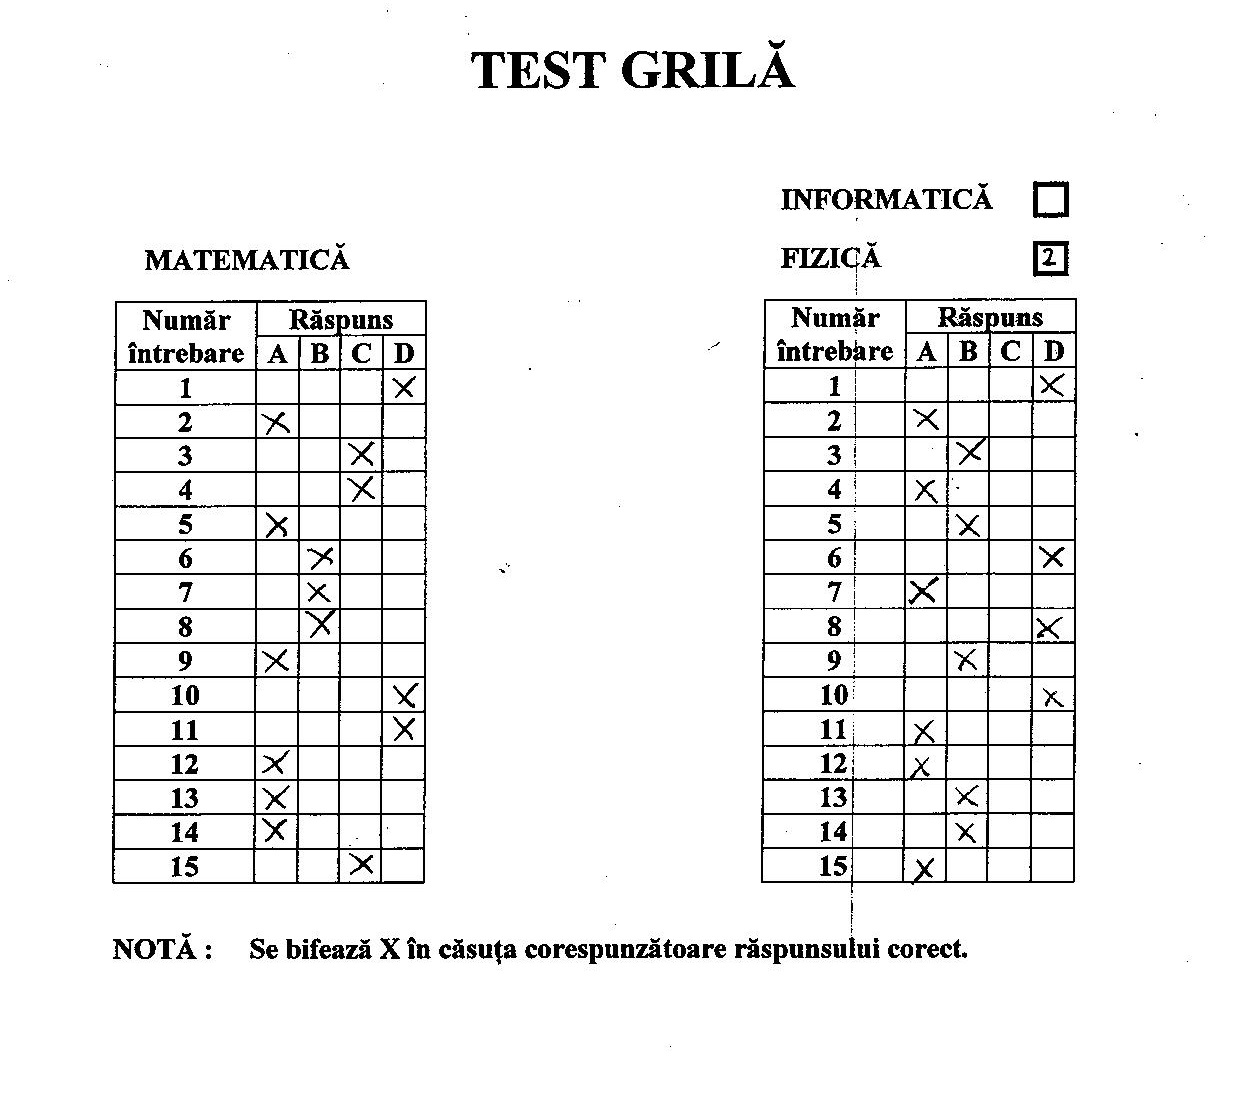
\includegraphics[width = 73mm]{fig3_5_1} 
		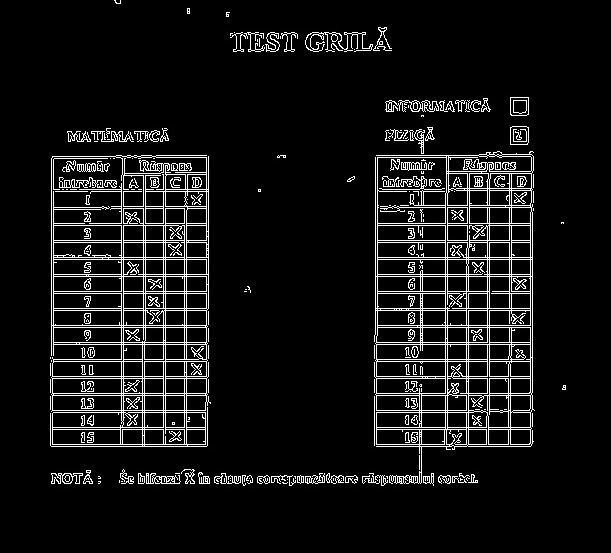
\includegraphics[width = 73mm]{fig3_5_2} \\
		\textbf  {Figura 3.5} Detecția muchiilor folosind Canny (imagine fără filtrul Gaussian)
	\end {footnotesize} 
\end {center}
\tab În urma detecției muchiilor pot rezulta în imagine zone de discontinuitate, astfel încât procesul de găsire a contururilor nu o să ofere ca răspuns grilele existente în lucrare. În vederea evitării acestui comportament, se aplică asupra imaginii o operație de închidere a muchiilor, fiind reprezentată de o transformare morfologică. De asemenea, răspunsul imaginii constă și în evidențierea mai exactă a muchiilor detectate cu ajutorul lui Canny. În figura 3.6 este prezentat rezultatul aplicării metodei de închidere, și totodată de accentuare a muchiilor asupra imaginii rezultate în urma detectorului Canny (în stânga este imaginea inițială, iar în dreapta imaginea după modificările aduse).
\begin {center} 
	\begin {footnotesize} 
		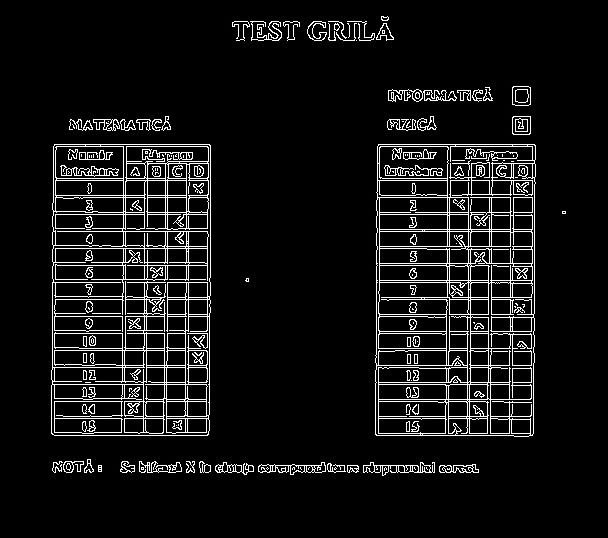
\includegraphics[width = 73mm]{fig3_6_1} 
		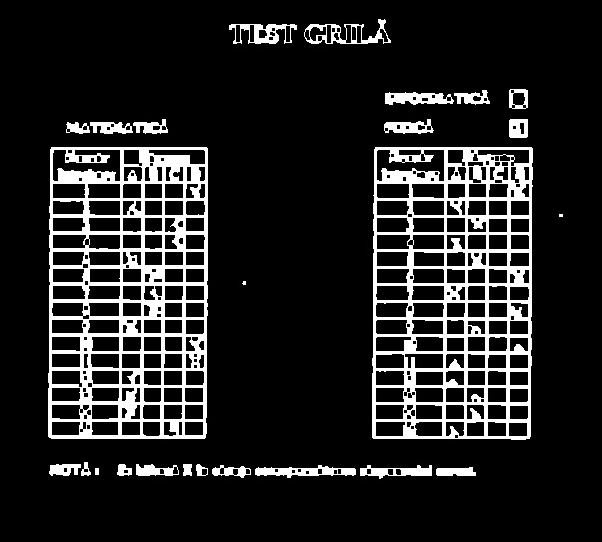
\includegraphics[width = 73mm]{fig3_6_2} \\
		\textbf  {Figura 3.6} Închiderea și evidențierea muchiilor folosind \\ operația morfologică de închidere
	\end {footnotesize} 
\end {center}
\tab Ultimul pas este reprezentat de detecția contururilor, în care se execută o operație de aproximare a muchiilor fiecărui contur, aplicând metoda Ramer-Douglas-Peucker. Ideea principală a aproximării este aceea că pentru orice curbă formată din mai multe segmente de dreaptă putem găsi o altă curbă formată din mai puține segmente. Această abordare este una utilă în sensul în care fiecare muchie a obiectelor existente în imagine este formată din mai multe segmente, care nu reprezintă muchii noi, ci doar deformări datorate imprimării, scanării și procesării imaginilor. În urma aproximării aplicate muchiilor existente în lucrare, grilele pe care dorim să le extragem vor avea 4 laturi, fapt evidențiat în figura 3.7 unde au fost reprezentate pe imagine doar contururile de 4 laturi care au fost detectate în imagine.
\begin {center} 
	\begin {footnotesize} 
		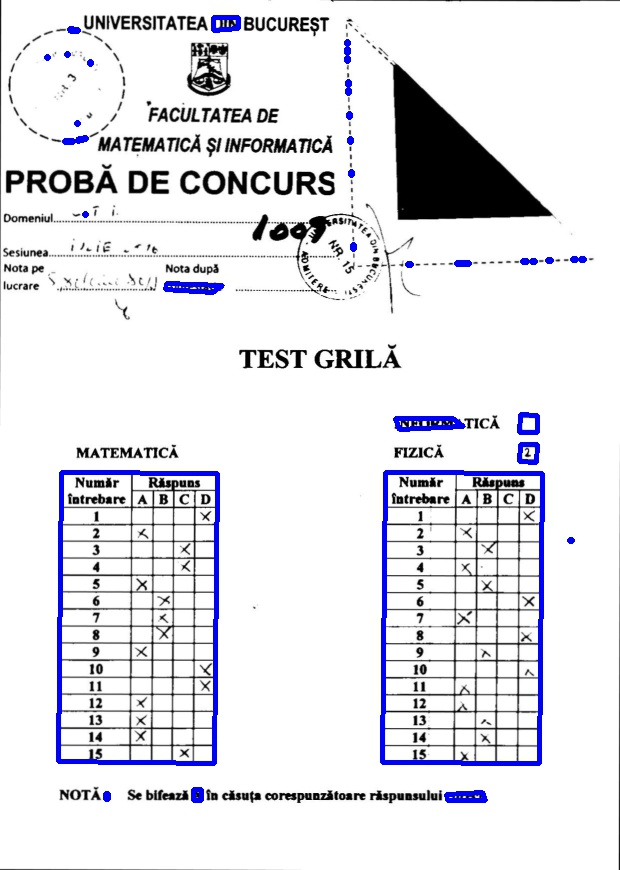
\includegraphics[width = 80mm]{fig3_7} \\
		\textbf  {Figura 3.7} Reprezentarea contururilor detectate
	\end {footnotesize} 
\end {center}
\tab În momentul printării și scanării lucrărilor, acestea pot suferi o rotire către stânga sau către dreapta. Pentru a corecta acest aspect se aplică o metodă de rotire în sens invers orientării pe care o are imaginea în momentul inițial. Această operație este executată folosind o matrice de rotație, obținută cu ajutorul unei funcții a cărei parametrii sunt reprezentați de punctul în jurul căruia se execută rotirea, caz în care se iau în considerare valorile centrului imaginii (înălțime imagine/2, lățime imagine/2), unghiul de rotire (o valoare pozitivă înseamnă în sensul acelor de ceasornic, iar o valoare negativă înseamnă în sens invers) și factorul de scalare al imaginii. Matricea astfel obținută reprezintă parametru de intrare pentru o transformare afină care va executa rotația. Transformarea afină\cite{opencv6} este reprezentată de o funcție care efectuează diverse transformări ale imaginilor 2D. Modificările aduse nu intervin asupra conținutului imaginii, ci schimbă poziția pixelilor, în vederea rotirii imaginii. 
\\ \tab Grilele existente în lucrările care se corectează au ariile cele mai mari comparativ cu restul obiectelor care au 4 laturi detectate de către metoda de găsire a contururilor. Astfel, se determină cele mai mari 2 arii ale patrulaterelor existente, iar coordonatele colțurilor acestora reprezintă valorile în funcție de care se decupează grilele din lucrare. Aria unui patrulater dat de punctele  ($x_{1}$,  $y_{1}$), ($x_{2}$,  $y_{2}$), ($x_{3}$,  $y_{3}$), ($x_{4}$,  $y_{4}$) este egală cu suma ariilor triunghiurilor formate de punctele ($x_{1}$,  $y_{1}$), ($x_{2}$,  $y_{2}$), ($x_{4}$,  $y_{4}$), respectiv  ($x_{2}$,  $y_{2}$), ($x_{3}$,  $y_{3}$), ($x_{4}$,  $y_{4}$). În plus, se execută operații de comparare a valorilor coordonatelor celor 8 colțuri detectate în urma procesului descris anterior, astfel încât la finalul etapei de extragere a grilelor, ordinea punctelor devine cea prezentată în figura 3.8.
\begin {center} 
	\begin {footnotesize} 
		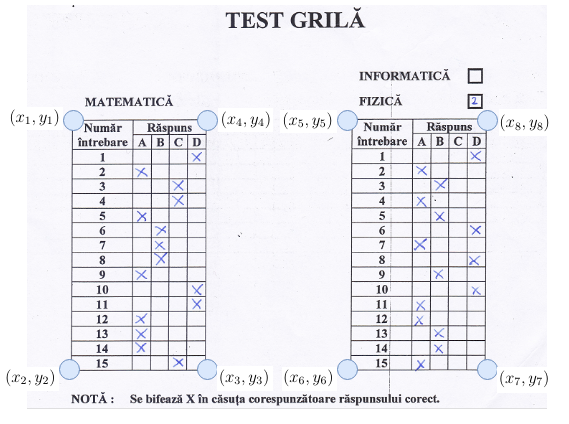
\includegraphics[height = 120mm, width =155mm]{fig3_8} \\
		\textbf  {Figura 3.8} Coordonatele obținute în urma \\ detecției colțurilor grilelor
	\end {footnotesize} 
\end {center}
\tab În figura 3.9 sunt prezentate grilele care au fost decupate din lucrarea care se corectează, conform modalităților descrise anterior.
\begin {center} 
	\begin {footnotesize} 
		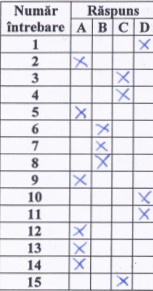
\includegraphics[width = 30mm]{fig3_9_1} 
		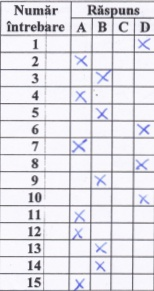
\includegraphics[width = 30mm]{fig3_9_2} \\
		\textbf  {Figura 3.9} Grilele care au fost decupate \\ din lucrare
	\end {footnotesize} 
\end {center}

\section{Determinarea răspunsurilor bifate}
\tab Grilele rezultate în urma procesului de extragere care a fost prezentat în secțiunea anterioară cuprind două parți, și anume: numărul întrebărilor (1-15), alături de posibilele răspunsuri pentru fiecare întrebare (A-D) și zona efectivă unde se vor bifa răspunsurile. Modulul descris în secțiunea de față are rolul de a oferi ca rezultat câte o matrice cu 15 rânduri și 4 coloane pentru fiecare dintre grilele de matematică și informatică/fizică în care elementele de pe pozițiile pe care se află o bifă a elevului să fie 1, iar restul 0. 
\\ \tab Primul pas realizat este acela de decupare a secțiunilor care nu fac parte din zona în care se găsesc bifele elevului. Se definește astfel o metodă care citește imaginea în care se află grila decupată și oferă ca răspuns doar zonele în care se găsesc răspunsurile care au fost selectate de elev. În figura 3.10 sunt prezentate cele două rezultate oferite de implementarea descrisă.
\begin {center} 
	\begin {footnotesize} 
		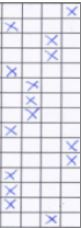
\includegraphics[width = 23mm]{fig3_10_1} 
		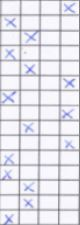
\includegraphics[width = 23mm]{fig3_10_2} \\
		\textbf  {Figura 3.10} Zonele cu răspunsuri din grilele extrase
	\end {footnotesize} 
\end {center}
\tab Imaginile rezultate în urma procesului de decupare parcurg o etapă de accentuare a muchiilor existente, dar și a bifelor elevului. Importanța acestei etape este aceea de evidențiere exactă a pozițiilor pe care se află răspunsurile. Pentru a se realiza acest pas, se aplică detectorul de muchii Canny, alături de metoda de închidere a muchiilor folosind transformarea morfologică. În figura 3.11 sunt prezentate răspunsurile metodei de accentuare a detaliilor zonelor cu răspunsuri. De asemenea, în urma acestei procesări zonele în care există bife  au o intensitate totală mare, datorită existenței culorii alb (valoarea 255), iar zonele în care nu există bife au o intensitate totală mică, datorită existenței culorii negru (valoarea 0).  
\begin {center} 
	\begin {footnotesize} 
		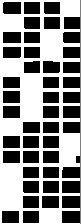
\includegraphics[width = 23mm]{fig3_11_1} 
		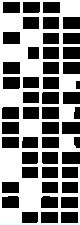
\includegraphics[width = 23mm]{fig3_11_2} \\
		\textbf  {Figura 3.11} Accentuarea detaliilor zonelor cu răspunsuri
	\end {footnotesize} 
\end {center}
\tab În vederea realizării matricei formată din 15 rânduri și 4 coloane, imaginea accentuată a zonei răspunsurilor este împărțită în 15 secțiuni egale, corespunzătoare tuturor întrebărilor existente. Fiecare astfel de secțiune rezultată este la rândul ei împărțită în 4 zone, datorită celor 4 răspunsuri posibile pentru fiecare întrebare în parte. Se determină care dintre cele 4 zone are intensitatea de culoare maximă, astfel încât poziția corespunzătoare maximului este reprezentată de poziția pe care se află răspunsul. De exemplu, pentru întrebarea 1, dacă poziția maximului este 1, înseamnă că intensitatea de culoare maximă este pe poziția 1, astfel încât rândul corespunzător matricei de răspunsuri va avea valoarea (1, 0, 0, 0). De asemenea, se verifică faptul că maximul găsit reprezintă o bifă,  existând posibilitatea ca în momentul în care o întrebare este lăsată necompletată, valoarea maximă determinată să fie o zonă în care există zgomot (trebuie îndeplinită condiția ca maximul găsit să aibă o valoare comparativ mai mare față de minimul calculat).
În figura 3.12 se prezintă zona de răspunsuri pentru o grilă existentă în lucrare, alături de matricea rezultată în urma aplicării metodei de determinare a răspunsurilor bifate.
\begin {center} 
	\begin {footnotesize} 
		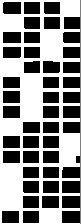
\includegraphics[width = 23mm]{fig3_12_1} 
		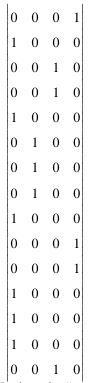
\includegraphics[height = 65mm,width = 20mm]{fig3_12_2} \\
		\textbf  {Figura 3.12}  Matricea de răspunsuri rezultată
	\end {footnotesize} 
\end {center}
\section {Determinarea tipului grilei completate și a numărului \\variantei primite}
\tab În urma extragerii grilelor prin determinarea valorilor perechilor de coordonate $(x, y)$ care aparțin colțurilor acestora, se poate decupa din lucrarea care se corectează, zona în care se găsesc bifele aferente tipului de subiect rezolvat și a numărului variantei primite de către elev. Această zonă este situată în apropierea coordonatelor $(x_{8}, y_{8})$, astfel încât se aplică o metodă de decupare a zonei respective, conform rezultatului prezentat în figura 3.13.  
\begin {center} 
	\begin {footnotesize} 
		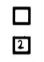
\includegraphics[width = 23mm]{fig3_13} \\
		\textbf  {Figura 3.13}  Zona aferentă tipului grilei și a numărului variantei
	\end {footnotesize} 
\end {center}
\tab În prima etapă se determină tipul de grilă care a fost rezolvat, adică informatică sau fizică. Analizarea zonei care a fost extrasă din lucrarea care se corectează, aferentă exemplului din figura 3.13, este similară cu metoda de detectare a răspunsurilor bifate. În acest sens, se accentuează detaliile existente în imagine prin aplicarea metodei de detectare a muchiilor și de închidere a acestora, rezultat care este reprezentat în figura 3.14. Totodată, imaginea este impărțită în 2 zone (informatică și fizică), pentru care se calculeaza intensitatea totală a culorilor. Zona în care intensitatea este maximă (pixeli albi) reprezintă zona în care a fost bifată opțiunea de grilă rezolvată, rezultatul metodei fiind reprezentat de un string a cărui valoare este ``informatică`` sau ``fizică``. Rezultatul metodei de detectare a tipului grilei pentru figura 3.14 este ``fizică``.
\begin {center} 
	\begin {footnotesize} 
		
\includegraphics[width = 23mm]{fig3_14} \\
		\textbf  {Figura 3.14}  Zona accentuată a tipului grilei 
	\end {footnotesize} 
\end {center}
\tab A doua etapă este reprezentată de detectarea numărului variantei primite de către elev. Ideea constă în antrenarea unui clasificator SVM folosind ca descriptor histogramele de gradienți orientați. Clasificarea imaginilor este realizată prin tehnica învățării supervizate și astfel, datele de ieșire sunt împărțite în diverse clase de obiecte. Datorită faptului că la examenul de admitere se propun 4 variante de subiecte (numerotate de la 1 la 4), etapele de antrenare și testare a clasificatorului se realizează pentru 4 clase de obiecte. 
\\ \tab Primul pas care se execută în vederea antrenării clasificatorului este reprezentat de parcurgerea celor 60.000 de imagini de antrenare ale setului de date MNIST. Dintre imaginile existente se aleg doar acele imagini a căror etichetă este 1, 2, 3 sau 4, astfel încât la finalul procesului de antrenare rezultă un clasificator pentru 4 clase de obiecte, și anume cifrele 1, 2, 3 și 4. Pentru fiecare astfel de imagine se calculează descriptorul HOG, urmând ca rezultatul să fie adăugat într-o listă de descriptori. În figura 3.15 sunt prezentate imagini ale cifrelor 1, 2, 3 și 4 din setul de date MNIST, alături de rezultatele calculării histogramelor de gradienți orientați pentru acestea (hog cu 4 ferestre a câte $14\times14$ pixeli fiecare).
\begin {center} 
	\begin {footnotesize} 
		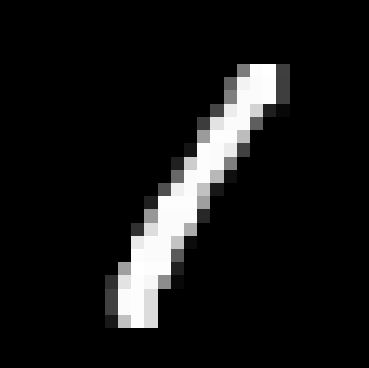
\includegraphics[width = 26mm]{fig3_15_1} 
		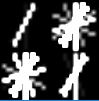
\includegraphics[width = 25mm]{fig3_15_2} 
		
\includegraphics[width = 26mm]{fig3_15_3} 
		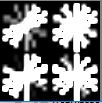
\includegraphics[width = 25mm]{fig3_15_4} \\
		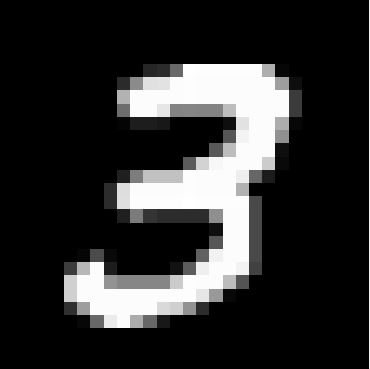
\includegraphics[width = 26mm]{fig3_15_5} 
		\includegraphics[width = 25mm]{fig3_15_6} 
		\includegraphics[width = 26mm]{fig3_15_7} 
		\includegraphics[width = 25mm]{fig3_15_8} \\
		\textbf  {Figura 3.15}  Rezultatul calculării HOG asupra imaginilor cu cifre
	\end {footnotesize} 
\end {center}
\tab În figura 3.16 se prezintă graficele cu valorile histogramelor calculate pentru imaginile din figura 3.15.
\begin {center} 
	\begin {footnotesize} 
		\includegraphics[width = 65mm]{fig3_16_1} 
		\includegraphics[width = 67mm]{fig3_16_2} 
		\includegraphics[width = 65mm]{fig3_16_3} 
		\includegraphics[width = 65mm]{fig3_16_4} \\
		\textbf  {Figura 3.16}  Graficele HOG-urilor aferente imaginilor din figura 3.15
	\end {footnotesize} 
\end {center}
\tab Descriptorii HOG astfel calculați reprezintă date de intrare pentru procesul de învățare supervizată, alături de etichetele corespunzătoare acestor histograme. Estimatorul metodei de clasificare a imaginilor este un obiect care implementează două funcții, \textit{fit} și \textit{predict}. Funcția \textit{fit} primește ca parametrii descriptorii setului de imagini de antrenare și etichetele acestora, realizând astfel modelul clasificatorului. Funcția \textit{predict} primește ca parametru o imagine și are rolul de a prezice eticheta pentru aceasta. În urma realizării procesului de învățare supervizată, modelul rezultat se salvează într-un fișier .pkl (pickle). 
\\ \tab Precizia clasificatorului se calculează folosind cele 10.000 de date de test oferite de setul MNIST. Astfel, se parcurg iterativ imaginile, iar pentru fiecare imagine se aplică metoda de clasificare. Rezultatele obținute sunt comparate cu etichetele corespunzătoare imaginilor de test și astfel se determină acuratețea modelului creat. Datele experimentale obținute în dezvoltarea clasificatorului sunt prezentate în capitolul următor. 
\\ \tab După antrenarea și testarea performanței clasificatorului, procesarea continuă prin extragerea cifrei corespunzătoare numărului variantei lucrării care se corectează. Această etapă se realizează prin detectarea contururilor obiectelor în imaginea care a fost decupată din apropierea coordonatelor colțului din dreapta sus (care aparține grilei de informatică-fizică, adică, $(x_{8}, y_{8})$), rezultat prezentat în figura 3.17. 
\begin {center} 
	\begin {footnotesize} 
		\includegraphics[width = 23mm]{fig3_17} \\
		\textbf  {Figura 3.17}  Contururile detectate în zona numărului variantei
	\end {footnotesize} 
\end {center}
\tab În urma detecției realizate se extrag cele două contururi care au perimetrul cel mai mare și se calculează valoarea totală a intensității de culoare pentru fiecare în parte. Pentru zonele corespunzătoare acestor contururi de perimetru maxim se aplică transformarea morfologică de închidere a muchiilor și de accentuare a detaliilor, astfel încât detecția bifei în care a fost completată cifra să fie realizată cu succes. Zona în care intensitatea totală este maximă, este reprezentată de existența cifrei care oferă numărul variantei de subiect din lucrarea care se corectează. Prin urmare, se salvează, în vederea procesării ulterioare, interiorul conturului corespunzător bifei de intensitate maximă. Imaginile rezultate în urma aplicării acestui pas asupra unor lucrări din setul de test sunt prezentate în figura 3.18.
\begin {center} 
	\begin {footnotesize} 
		\includegraphics[width = 18mm]{fig3_18_1} 
		\includegraphics[width = 18mm]{fig3_18_2} 
		\includegraphics[width = 18mm]{fig3_18_3} 
		\includegraphics[width = 18mm]{fig3_18_4} \\
		\textbf  {Figura 3.18} Cifre extrase din lucrări ale setului de test
	\end {footnotesize} 
\end {center} 
\tab Ultima etapă realizată în determinarea numărului variantei este aceea de prezicere a cifrei extrase din lucrare prin aplicarea metodei \textit{predict}. Astfel, imaginea corespunzătoare cifrei (conform figurii 3.18) este transformată din RGB în tonuri de gri și i se aplică descriptorul HOG în același mod în care s-a aplicat setului de date de antrenare. Rezultatul este reprezentat de o etichetă a cărei valoare poate fi 1, 2, 3 sau 4. 
\section{Compararea răspunsurilor bifate cu cele corecte}
\tab În urma detectării tipului grilei rezolvate și a numărului variantei primite de către elev, se realizează comparații între matricele rezultate din lucrarea care se corectează și matricele de răspunsuri introduse de către comisia de admitere. Această etapă este efectuată prin definirea unei metode care parcurge în paralel o matrice de răspunsuri determinată în urma procesării lucrării elevului și matricea corespunzătoare acesteia, care a fost introdusă în aplicație. Dacă în urma procesului de detectare a numărului variantei și a tipului acesteia rezultă că elevul a primit setul de subiecte cu numărul 2 și a rezolvat grila de fizică, se parcurg în paralel matricele obținute prin analizarea, respectiv procesarea lucrării și cele aferente grilelor de matematică și fizică varianta 2, introduse în aplicație.
\\ \tab Metoda descrisă parcurge în paralel cele două matrice primite ca parametru și verifică câte linii din aceste matrice sunt identice. Numărul astfel rezultat reprezintă numărul de răspunsuri care au fost bifate corect de către elev în grila respectivă. În figura 3.19 se prezintă matricea de răspunsuri pentru grila de matematică varianta 2 introdusă de către comisia de admitere (în stânga) și matricea de răspunsuri a elevului (în dreapta), iar rezultatul procesului descris la această etapă este 8, reprezentând numărul de răspunsuri bifate corect.
\begin {center} 
	\begin {footnotesize} 
		\includegraphics[width = 53mm]{fig3_19} \\
		\textbf  {Figura 3.19} Compararea răspunsurilor bifate cu cele corecte
	\end {footnotesize} 
\end {center}
\section{Determinarea notei finale}
\tab În urma comparării matricelor de răspunsuri obținute din lucrarea care se procesează cu matricele introduse de către comisia de admitere, rezultă două valori care semnifică numărul de răspunsuri la grila de matematică, respectiv numărul de răspunsuri la grila de informatică sau fizică. În funcție de aceste valori se calculează nota finală a lucrării, după formula: 0.3p * (număr răspunsuri la grila de matematică + număr răspunsuri la grila de informatică sau fizică) + 1p (oficiu). Notele determinate pentru lucrările corectate se scriu într-un fișier text și pot fi analizate de către comisia de admitere. De asemenea, pentru fiecare lucrare se scriu în fișier informații necesare despre aceasta, precum tipul grilei completate, numărul variantei care a fost detectat folosind clasificatorul antrenat și numărul de răspunsuri pentru fiecare grilă în parte.
\section{Testarea funcționalităților implementate}
\tab Testarea unei aplicații software reprezintă o componentă importantă a procesului de dezvoltare, care oferă informații cu privire la calitatea și funcționarea în parametrii optimi a soft-ului creat. 
\\ \tab Aplicația prezentată în lucrarea de față a fost testată folosind un număr de 191 de lucrări  care au fost completate și corectate la examenul de admitere din iulie 2016.
\\ \tab Componenta de testare a fost realizată prin crearea unei suite de teste unitare, care parcurg următorii pași:
\begin{itemize}
\setlength\itemsep{1pt}
\item reducerea zgomotului din lucrările care se corectează
\item extragerea grilelor din lucrare și determinarea matricelor de răspunsuri corespunzătoare acestora
\item determinarea tipului de grilă care a fost completat (informatică sau fizică)
\item calcularea notei finale conform formulei care a fost descrisă în secțiunea 3.5
\item compararea tipului de grilă determinat automat de aplicație, cu cel existent în lucrare
\item compararea notei finale obținută de aplicație cu nota scrisă pe foaia de examen (matricele detectate se compară cu valori ale matricelor setate implicit, fără a se detecta automat numărul variantei primite de către elev).
\end{itemize}
\tab Rezultatele obținute în timpul procesului de testare sunt prezentate în capitolul următor. 
\section{Realizarea interfeței cu utilizatorul}
\tab Realizarea interfeței grafice este etapa în care toate funcționalitățile prezentate în capitolul de față devin accesibile pentru utilizatorul aplicației. Aceste funcționalități sunt:
\begin{itemize}
\setlength\itemsep{1pt}
\item introducerea valorii pragului de eliminare a zgomotului (valoarea optimă este 180)
\item evaluarea unui set de lucrări completate de către elevi cu detectarea automată a tipului grilei și a variantei primite 
\item evaluarea unui set de lucrări pentru care se selectează tipul grilei și varianta primită
\item rularea testelor automate
\item adăugarea răspunsurilor de către comisia de admitere
\item corectarea unei lucrări și încercuirea cu roșu sau verde a răspunsului în funcție de corectitudinea acestuia.
\end{itemize}
\section{Tehnologii folosite}
\tab Dezvoltarea aplicației descrise în prezenta lucrare a fost realizată folosind limbajul de programare Python, fiind un limbaj utilizat într-o mare varietate de aplicații, proiectat de Guido van
Rossum și dezvoltat de compania Python Software Foundation. Avantajul major îl reprezintă faptul că Python este un limbaj de scripting, astfel încât codul scris se interpretează, nu se compilează, de aici rezultând un timp redus în 
dezvoltarea și testarea aplicațiilor. Mediul de dezvoltare folosit este Pycharm, iar proiectul este stucturat în mai multe fișiere care se numesc scripturi cu extensia .py. De asemenea, s-au utilizat un set de biblioteci, și anume:
\begin{enumerate}
\setlength\itemsep{1pt}
\item NumPy - manipularea structurilor de date de dimensiuni mari (vectori și matrice)
\item Tkinter - crearea interfeței cu utilizatorul aplicației
\item UnitTest - crearea testelor unitare în vederea verificării funcționalităților aplicației
\item OpenCV - dezvoltarea aplicațiilor de vedere artificială (afișare imagini digitale, filtrare, redimensionare, transformări morfologice)
\item Scikit-Learn - dezvoltarea aplicațiilor de machine learning (clasificare, regresie, clusterizare)
\item SciPy - utilizat în calculul științific (algebră liniară, optimizare, procesarea imaginilor).
\end{enumerate}


\chapter*{}

\chapter{Rezultate experimentale}
\tab Funcționalitățile aplicației descrise în prezenta lucrare au fost testate folosind un set de 191 de lucrări de la examenul de admitere din sesiunea iulie 2016, care au fost scanate. Rezultatele experimentale efectuate asupra aplicației sunt împărțite în mai multe secțiuni, și anume:
\begin{enumerate}
\setlength\itemsep{1pt}
\item verificarea pragului de eliminare al zgomotului
\item timpul mediu de execuție al corectării
\item rularea testelor unitare
\item acuratețea clasificatorului liniar SVM folosind HOG cu dimensiunea de 4 celule
\item acuratețea clasificatorului liniar SVM folosind HOG cu dimensiunea de 16 celule.
\end{enumerate}

\subsection*{\centering 1. Verificarea pragului de eliminare al zgomotului}
\tab În vederea testării valorilor parametrului în funcție de care se realizează eliminarea zgomotului, se aplică această metodă pentru un set de imagini scanate, iar răspunsurile sunt prezentate în tabelul 4.1. 
\begin{center}
\begin{tabu} to 0.8\textwidth { | X[c] | X[c] | }
 \hline
 \textbf{Valoare} & \textbf{Detectare corectă a grilelor} \\
 \hline
 0$<$passFactor$<$150  & Nu \\
\hline
 150$\leq$passFactor$\leq$200  & Da \\
\hline
200$<$passFactor$\leq$255  & Nu \\
\hline
\end{tabu}
\begin {footnotesize} 
\\ \tab \\ \textbf  {Tabelul 4.1} Verificarea valorilor pragului de eliminare al zgomotului
\end {footnotesize} 
\end{center}
\tab În urma aplicării diverselor praguri de eliminare al zgomotului se observă că valorile optime pentru care detecția grilelor este realizată în mod corespunzător sunt situate în intervalul 150-200.

\subsection*{\centering 2. Timpul mediu de execuție al corectării}
\tab În prezenta secțiune se analizează timpul de execuție al corectării lucrărilor scanate, folosind un prag de eliminare al zgomotului cu valoarea de 180 (tabelul 4.2).
\begin{center}
\begin{tabu} to 0.8\textwidth { | X[c] | X[c] | }
 \hline
 \textbf{Număr imagini} & \textbf{Timpul mediu de execuție } \\
 \hline
 1  & 7.8-8.3 secunde \\
\hline
 191  & 24.83-26.42 minute \\
\hline
\end{tabu}
\begin {footnotesize} 
\\ \tab \\ \textbf  {Tabelul 4.2} Timpul mediu de execuție al corectării
\end {footnotesize} 
\end{center}
\tab În tabelul 4.3 se prezintă timpul de execuție pentru fiecare pas realizat în procesul automat de corectare al unei singure lucrări scanate, folosind un prag de eliminare al zgomotului cu valoarea de 180.
\begin{center}
\begin{tabu} to 0.8\textwidth { | X[c] | X[c] | }
 \hline
 \textbf{Pasul realizat} & \textbf{Timpul mediu de execuție } \\
 \hline
 scanare lucrare  & 10 secunde \\
\hline
 introducere răspunsuri corecte  & 1 minut \\
\hline
eliminare zgomot & 6.5-7.8 secunde \\
\hline
extragere grile & 0.37-0.9 secunde \\
\hline
determinare tip grilă +  nr var& 0.59-0.73 secunde \\
\hline
determinare răspunsuri bifate & 0.06-0.078 secunde \\
\hline
calculare notă & 0.001 secunde \\
\hline
\end{tabu}
\begin {footnotesize} 
\\ \tab \\ \textbf  {Tabelul 4.3} Timpul mediu de execuție al întregului proces pentru o lucrare
\end {footnotesize} 
\end{center}

\subsection*{\centering 3. Rularea testelor unitare}
\tab Suita de teste unitare creată pentru întreg setul de lucrări a rulat cu succes pentru valorile pragului de eliminare al zgomotului care au fost prezentate în tabelul 4.1 și care produc detecția grilelor într-un mod corespunzător (valori între 150 și 200). În decursul procesului de testare au fost verificate valorile aferente tipului de grilă care a fost rezolvat de către elev și a notei finale obținute, care a fost comparată cu nota existentă pe lucrarea corectată la admiterea din iulie 2016. Matricele de răspunsuri corecte cu ajutorul cărora s-au calculat notele finale au fost setate implicit ca parametrii de intrare metodelor de determinare a rezultatelor, fără a se detecta automat numărul subiectului primit de către elev și, astfel, a matricelor corespunzătoare. Datorită faptului că nu s-a apelat metoda predict a estimatorului, pentru determinarea numărului variantei de subiect, timpii de execuție ai testelor sunt mai reduși, conform datelor prezentate în tabelul 4.4.
\begin{center}
\begin{tabu} to 0.8\textwidth { | X[c] | X[c] | }
 \hline
 \textbf{Număr teste} & \textbf{Timpul mediu de execuție} \\
 \hline
 1  & 7.5-7.7 secunde \\
\hline
 191  & 23.87-24.51 minute \\
\hline
\end{tabu}
\begin {footnotesize} 
\\ \tab \\ \textbf  {Tabelul 4.4} Timpul mediu de execuție al testelor
\end {footnotesize} 
\end{center}
\subsection*{\centering 4. Acuratețea clasificatorului liniar SVM folosind HOG\\ cu dimensiunea de 4 celule}
\tab În vederea antrenării clasificatorului SVM se folosește ca descriptor histogramele de gradienți orientați cu o dimensiune a caroiajului de 4 celule. Setul de date de antrenare este reprezentat de MNIST, din care se utilizează doar imaginile cu cifre de 1, 2, 3 și 4. De asemenea, se analizează acuratețea modelului creat folosind două seturi de date de test: imagini cu cifre aparținând setului de date MNIST (figura 4.1) și imagini cu cifre aparținând lucrărilor completate la examenul de admitere din iulie 2016 (figura 4.2).
\begin {center} 
	\begin {footnotesize} 
		\includegraphics[width = 85mm]{fig2_15} \\
		\textbf  {Figura 4.1} Imagini cu cifre din setul MNIST
	\end {footnotesize} 
\end {center}

\begin {center} 
	\begin {footnotesize} 
		\includegraphics[width = 17mm]{fig3_18_1} 
		\includegraphics[width = 17mm]{fig3_18_2} 
		\includegraphics[width = 17mm]{fig3_18_3} 
		\includegraphics[width = 17mm]{fig3_18_4} \\
		\textbf  {Figura 4.2} Imagini cu cifre din lucrări completate la examenul de admitere din iulie 2016
	\end {footnotesize} 
\end {center} 
\tab În tabelul 4.5 se prezintă acuratețea clasificatorului SVM folosind histograme de gradienți orientați cu dimensiunea caroiajului de 4 celule, antrenat pe un număr diferit de imagini din setul MNIST și testat folosind imagini din același set. 
\begin{center}
\begin{tabu} to 0.8\textwidth { | X[c] | X[c] | X[c] |}
 \hline
 \textbf{Nr img antenare MNIST} & \textbf{Nr img testare MNIST} & \textbf{Acuratețe} \\
 \hline
 100  & 4159  & 89.3\% \\
 \hline
 1000  & 4159  & 93.75\% \\
\hline
 10000  & 4159  & 94.81\% \\
 \hline
 24673  & 4159  & 94.85\% \\
\hline
\end{tabu}
\begin {footnotesize} 
\\ \tab \\ \textbf  {Tabelul 4.5} Acuratețe SVM folosind HOG 4 celule - teste MNIST
\end {footnotesize} 
\end{center}
\tab În tabelul 4.6 se prezintă acuratețea clasificatorului SVM folosind histograme de gradienți orientați cu dimensiunea caroiajului de 4 celule, antrenat pe un număr diferit de imagini din setul MNIST și testat folosind imagini ale lucrărilor completate la examenul de admitere din iulie 2016.
\begin{center}
\begin{tabu} to 0.8\textwidth { | X[c] | X[c] | X[c] |}
 \hline
 \textbf{Nr img antenare MNIST} & \textbf{Nr img testare lucrări 2016} & \textbf{Acuratețe} \\
 \hline
 100  & 191  & 72.25\% \\
 \hline
 1000  & 191  & 78.01\% \\
\hline
 10000  & 191  & 80.01\% \\
 \hline
 24673  & 191  & 79.58\% \\
\hline
\end{tabu}
\begin {footnotesize} 
\\ \tab \\ \textbf  {Tabelul 4.6} Acuratețe SVM folosind HOG 4 celule - teste lucrări 2016
\end {footnotesize} 
\end{center}
\tab În tabelul 4.7 se prezintă timpul de execuție necesar antrenării, respectiv testării clasificatorului SVM folosind histograme de gradienți orientați cu dimensiunea caroiajului de 4 celule. Pentru antrenare se folosesc un număr diferit de imagini din setul MNIST, iar pentru procesul de testare se folosesc imagini din același set.
\begin{center}
\begin{tabu} to 0.8\textwidth { | X[c] | X[c] | X[c] | X[c]|}
 \hline
 \textbf{Nr antenare MNIST} &  \textbf{Timp antrenare} & \textbf{Nr testare MNIST} & \textbf{Timp testare} \\
 \hline
 100  & 0.15-0.25 secunde & 4159  & 1.2-1.75 secunde \\
 \hline
 1000  & 0.4-0.55 secunde & 4159  & 1.7-1.85 secunde \\
\hline
 10000  & 4.01-4.55 secunde & 4159  & 2.02-2.35 secunde \\
 \hline
 24673  & 11.5-12.55 secunde & 4159  & 2.1-2.65 secunde \\
\hline
\end{tabu}
\begin {footnotesize} 
\\ \tab \\ \textbf  {Tabelul 4.7} Timpi de execuție antrenare MNIST și testare MNIST
\end {footnotesize} 
\end{center}
\tab În tabelul 4.8 se prezintă timpul de execuție necesar antrenării, respectiv testării clasificatorului SVM folosind histograme de gradienți orientați cu dimensiunea caroiajului de 4 celule. Pentru antrenare se folosesc un număr diferit de imagini din setul MNIST, iar pentru procesul de testare se folosesc imagini ale lucrărilor completate la examenul de admitere din iulie 2016.
\begin{center}
\begin{tabu} to 0.8\textwidth { | X[c] | X[c] | X[c] | X[c]|}
 \hline
 \textbf{Nr antenare MNIST} &  \textbf{Timp antrenare} & \textbf{Nr testare lucrări 2016} & \textbf{Timp testare} \\
 \hline
 100  & 0.15-0.25 secunde & 191  & 0.85-1.01 secunde \\
 \hline
 1000  & 0.4-0.55 secunde & 191  & 1.03-1.25 secunde \\
\hline
 10000  & 4.01-4.55 secunde & 191  & 2.1-2.35 secunde \\
 \hline
 24673  & 11.5-12.55 secunde & 191  & 3.05-3.65 secunde \\
\hline
\end{tabu}
\begin {footnotesize} 
\\ \tab \\ \textbf  {Tabelul 4.8} Timpi de execuție antrenare MNIST și testare lucrări 2016
\end {footnotesize} 
\end{center}

\subsection*{\centering Acuratețea clasificatorului liniar SVM folosind HOG\\ cu dimensiunea de 16 celule}
\tab În vederea obținerii unui clasificator care oferă o acuratețe mai mare, se mărește numărul de celule al HOG. Astfel, se folosește ca descriptor histogramele de gradienți orientați cu o dimensiune a caroiajului de 16 celule. Seturile de date necesare antrenării și testării clasificatorului sunt similare cu cele descrise în secțiunea precedentă.  
\\ \tab În tabelul 4.9 se prezintă acuratețea clasificatorului SVM folosind histograme de gradienți orientați cu dimensiunea caroiajului de 16 celule, antrenat pe un număr diferit de imagini din setul MNIST și testat folosind imagini din același set. 
\begin{center}
\begin{tabu} to 0.8\textwidth { | X[c] | X[c] | X[c] |}
 \hline
 \textbf{Nr img antenare MNIST} & \textbf{Nr img testare MNIST} & \textbf{Acuratețe} \\
 \hline
 100  & 4159  & 94.97\% \\
 \hline
 1000  & 4159  & 97.55\% \\
\hline
 10000  & 4159  & 99.3\% \\
 \hline
 24673  & 4159  & 99.3\% \\
\hline
\end{tabu}
\begin {footnotesize} 
\\ \tab \\ \textbf  {Tabelul 4.9} Acuratețe SVM folosind HOG 16 celule - teste MNIST
\end {footnotesize} 
\end{center}
\tab În tabelul 4.10 se prezintă acuratețea clasificatorului SVM folosind histograme de gradienți orientați cu dimensiunea caroiajului de 16 celule, antrenat pe un număr diferit de imagini din setul MNIST și testat folosind imagini ale lucrărilor completate la examenul de admitere din iulie 2016.
\begin{center}
\begin{tabu} to 0.8\textwidth { | X[c] | X[c] | X[c] |}
 \hline
 \textbf{Nr img antenare MNIST} & \textbf{Nr img testare lucrări 2016} & \textbf{Acuratețe} \\
 \hline
 100  & 191  & 67.54\% \\
 \hline
 1000  & 191  & 76.44\% \\
\hline
 10000  & 191  & 85.86\% \\
 \hline
 24673  & 191  & 85.86\% \\
\hline
\end{tabu}
\begin {footnotesize} 
\\ \tab \\ \textbf  {Tabelul 4.10} Acuratețe SVM folosind HOG 16 celule - teste lucrări 2016
\end {footnotesize} 
\end{center}
\tab În tabelul 4.11 se prezintă timpul de execuție necesar antrenării, respectiv testării clasificatorului SVM folosind histograme de gradienți orientați cu dimensiunea caroiajului de 16 celule. Pentru antrenare se folosesc un număr diferit de imagini din setul MNIST, iar pentru procesul de testare se folosesc imagini din același set.
\begin{center}
\begin{tabu} to 0.8\textwidth { | X[c] | X[c] | X[c] | X[c]|}
 \hline
 \textbf{Nr antenare MNIST} &  \textbf{Timp antrenare} & \textbf{Nr testare MNIST} & \textbf{Timp testare} \\
 \hline
 100  & 0.1-0.25 secunde & 4159  & 2.1-2.35 secunde \\
 \hline
 1000  & 0.5-0.75 secunde & 4159  & 2.5-2.85 secunde \\
\hline
 10000  & 21.01-22.3 secunde & 4159  & 4.07-5.25 secunde \\
 \hline
 24673  & 22.05-23.2 secunde & 4159  & 5.02-5.63 secunde \\
\hline
\end{tabu}
\begin {footnotesize} 
\\ \tab \\ \textbf  {Tabelul 4.11} Timpi de execuție antrenare MNIST și testare MNIST
\end {footnotesize} 
\end{center}

\tab În tabelul 4.12 se prezintă timpul de execuție necesar antrenării, respectiv testării clasificatorului SVM folosind histograme de gradienți orientați cu dimensiunea caroiajului de 16 celule. Pentru antrenare se folosesc un număr diferit de imagini din setul MNIST, iar pentru procesul de testare se folosesc imagini ale lucrărilor completate la examenul de admitere din iulie 2016.

\begin{center}
\begin{tabu} to 0.8\textwidth { | X[c] | X[c] | X[c] | X[c]|}
 \hline
 \textbf{Nr antenare MNIST} &  \textbf{Timp antrenare} & \textbf{Nr testare lucrări 2016} & \textbf{Timp testare} \\
 \hline
 100  & 0.1-0.25 secunde & 191  & 1.1-1.25 secunde \\
 \hline
 1000  & 0.5-0.75 secunde & 191  & 1.5-1.85 secunde \\
\hline
 10000  & 21.01-22.3 secunde & 191  & 6.15-6.75 secunde \\
 \hline
 24673  & 22.05-23.2 secunde & 191  & 6.15-6.85 secunde \\
\hline
\end{tabu}
\begin {footnotesize} 
\\ \tab \\ \textbf  {Tabelul 4.12} Timpi de execuție antrenare MNIST și testare lucrări 2016
\end {footnotesize} 
\end{center}
\tab În urma rezultatelor experimentale, observăm faptul că etapa de antrenare a unui clasificator SVM folosind un număr mai mare de celule pentru histogramele de gradienți orientați necesită un timp mai îndelungat de execuție, însă modelul creat oferă o acuratețe mai bună. 
În momentul în care se folosește un număr de celule mai mare pentru caroiajul HOG-urilor se calculează mai multe orientări ale pixelilor care formează o anumită cifră, și astfel clasificarea poate conduce la un rezultat mai exact. În figura 4.3 este prezentată diferența dintre rezultatele detecției folosind histograme cu un caroiaj de 4 celule, respectiv 16 celule, a unor cifre din setul de lucrări din iulie 2016. 
\begin {center} 
	\begin {footnotesize} 
		\includegraphics[width = 22mm]{fig4_3_1} 
		\includegraphics[width = 24mm]{fig4_3_2} 
		\includegraphics[width = 22mm]{fig4_3_3} \\
		\textbf {Etichetă imagine 1, HOG 4 celule - detecție 4, HOG 16 celule - detecție 1} \\
		\includegraphics[width = 22mm]{fig4_3_4} 
		\includegraphics[width = 22mm]{fig4_3_5} 
		\includegraphics[width = 22mm]{fig4_3_6}  \\
		\textbf {Etichetă imagine 3, HOG 4 celule - detecție 2, HOG 16 celule - detecție 3} \\
		\textbf  {Figura 4.3} Diferența dintre HOG 4 celule și 16 celule
	\end {footnotesize} 
\end {center}


\chapter*{}

\chapter{Concluzii}
\tab În urma analizării performanțelor aplicației se observă faptul că procesul automat de corectare durează în medie 2 ore și 10 minute pentru un set de 1000 de lucrări în format digital. Trebuie adăugat însă și timpul necesar scanării lucrărilor, și astfel să presupunem că sunt necesare 4 ore pentru finalizarea procesului de corectare. Aceste estimări sunt realizate fără a lua în calcul eroarea de 14.14\% care apare în momentul detectării numărului variantei care a fost rezolvat într-o anumită lucrare. De asemenea, în urma experimentelor realizate se observă faptul că antrenarea unui clasificator SVM liniar folosind un descriptor HOG cu mai multe celule necesită mai mult timp de execuție, însă oferă o acuratețe mult mai bună. 
\\ \tab Pentru a evita eroarea care apare în momentul detectării automate a numărului lucrării a fost adăugată în aplicație funcționalitatea prin care se poate alege manual tipul subiectului rezolvat în lucrare și astfel, precizia detectării corecte a notelor este de 100\%. Această abordare implică o mai mare activitate a comisiei de admitere care ar trebui sa sorteze lucrările în funcție de grila rezolvată, dar și de numărul subiectului primit și scanarea lor separată, procesul de corectare fiind executat pentru fiecare set de lucrări în parte.
\\ \tab În vederea obținerii unui factor de acuratețe ridicat se poate utiliza pentru antrenarea modelului o rețea neuronală, dar datorită complexității noțiunilor, acest tip de antrenare nu a fost cuprins în prezenta lucrare. De asemenea, pentru îmbunătățirea timpului de execuție a procesului automat se pot folosi mai multe fire de execuție care rulate în paralel realizează sarcinile necesare pentru obținerea rezultatului final.


\chapter*{}

\begin{thebibliography}{9}
\bibitem{articol1}
Francisco de Assis Zampirolli, Jose Artur Quilici Gonzalez, Rogerio Perino de Oliveira Neves. \textit{Automatic Correction of Multiple-Choice Tests using Digital Cameras and Image Processing}. \\
\href{http://iris.sel.eesc.usp.br/wvc/Anais_WVC2013/Poster/1/9.pdf}{http://iris.sel.eesc.usp.br/wvc/Anais\_WVC2013/Poster/1/9.pdf}
\bibitem{articol2}
Soumitra Patole, Aniket Pawar, Avanish Patel, Akshay Panchal, Prof. Ravindra Joshi. \textit{Automatic system for grading multiple choice questions and feedback analysis}. \\
\href{http://www.ijtra.com/special-issue-view/automatic-system-for-grading-multiple-choice-questions-and-feedback-analysis.pdf}{http://www.ijtra.com/special-issue-view/automatic-system-for-grading-multiple-choice-questions-and-feedback-analysis.pdf}
\bibitem{book1} 
Torras Carme. \textit{Computer Vision: Theory and Industrial Applications}. Springer-Verlag, 1992.
\bibitem{book2} 
Szeliski Richard. \textit{Computer Vision: Algorithms and Applications}. Springer, 2010.
\bibitem{opencv1} 
Morphological Transformations. \\
\href{http://docs.opencv.org/trunk/d9/d61/tutorial_py_morphological_ops.html}{http://docs.opencv.org/trunk/d9/d61/tutorial\_py\_morphological\_ops.html}
\bibitem{opencv2} 
Contours : Getting Started. \\
\href{http://docs.opencv.org/trunk/d4/d73/tutorial\_py\_contours\_begin.html}{http://docs.opencv.org/trunk/d4/d73/tutorial\_py\_contours\_begin.html}
\bibitem{wikip1} 
Prasad, Dilip K.; Leung, Maylor K.H.; Quek, Chai; Cho, Siu-Yeung. \textit{A novel framework for making dominant point detection methods non-parametric. Image and Vision Computing}. paginile: 843–859\\
\href{http://www.sciencedirect.com/science/article/pii/S0262885612000984}{http://www.sciencedirect.com/science/article/pii/S0262885612000984}
\bibitem{opencv3} 
Histogram of Oriented Gradients. \\
\href{http://www.learnopencv.com/histogram-of-oriented-gradients}{http://www.learnopencv.com/histogram-of-oriented-gradients}
\bibitem{opencv4} 
Histogram of Oriented Gradients (HOG) Descriptor. \\
\href{https://software.intel.com/en-us/node/529070}{https://software.intel.com/en-us/node/529070}
\bibitem{opencv5} 
Histogram of Oriented Gradients. \\
\href{http://scikit-image.org/docs/dev/auto\_examples/features\_detection/plot\_hog.html}{http://scikit-image.org/docs/dev/auto\_examples/features\_detection/plot\_hog.html}
\bibitem{wikip2} 
Theodoridis Sergios, Koutroumbas Konstantinos. \textit{Pattern recognition, second edition}. Elsevier Academic Press, 2003.
\bibitem{wikip3} 
Kecman Vojislav. \textit{Learning and Soft Computing: Support Vector Machines, Neural Networks, and Fuzzy Logic Models}. MIT Press, 2001.
\bibitem{sklearn} 
Support Vector Machines. \\
\href{http://scikit-learn.org/stable/modules/svm.html}{http://scikit-learn.org/stable/modules/svm.html}
\bibitem{mnist1} 
Visualizing MNIST: An Exploration of Dimensionality Reduction.
\href{http://colah.github.io/posts/2014-10-Visualizing-MNIST}{http://colah.github.io/posts/2014-10-Visualizing-MNIST}
\bibitem{wikip4} 
Mohri Mehryar, Rostamizadeh Afshin, Talwalkar Ameet. \textit{Foundations of Machine Learning}. The MIT Press, 2012.
\bibitem{opencv6} 
Geometric Image Transformations. \\
\href{http://docs.opencv.org/2.4/modules/imgproc/doc/geometric\_transformations.html?\\highlight=warpaffine}{http://docs.opencv.org/2.4/modules/imgproc/doc/geometric\_transformations.html?\\highlight=warpaffine}




\end{thebibliography}

\end{document}


















